% settings
%opening
\chapter{Qucs-S: Getting started analog simulation}

\hfill\textsl{This chapter is authored by Vadim Kuznetsov}

\section{Introduction} \label{sec:intro}

Qucs-S was forked from the Qucs cross-platform circuit simulator in 2017. "S" letter indicates SPICE. The purpose of the Qucs-S subproject is to use free SPICE circuit simulation kernels with the Qucs GUI. It merges the power of SPICE and the simplicity of the Qucs GUI. Qucs intentionally uses its own SPICE incompatible simulation kernel Qucsator. It has advanced RF and AC domain simulation features, but most of the existing industrial SPICE models are incompatible with it. Qucs-S is not a simulator by itself, but requires to use a simulation backend with it. The schematic document format of Qucs and Qucs-S are fully compatible. Qucs-S allows to use the following simulation kernels with it:

\begin{itemize}
 \item  Ngspice is recommended to use. Ngspice is powerful mixed-level/mixed-signal circuit simulator. The most of industrial SPICE models are compatible with Ngspice. It has an excellent performance for time-domain simulation of switching circuits and powerful postprocessor.
 \item XYCE is a new SPICE-compatible circuit simulator written by Sandia from the scratch.
 \item SpiceOpus is developed by the Faculty of Electrical Engineering of the Ljubljana University. It based on the SPICE-3f5 code.
 \item QucsatorRF for RF simulation with microwave devices and microstrip lines. It is not a SPICE compatible simulator. Not recommended for general purpose circuits.
\end{itemize}

Qucs-S is a cross-platform software and supports a number of Linux distributions alongside with Windows\texttrademark. The Linux packages are generated automatically with the Open Build Service (OBS ) system. Check the official website to get the list of supported distributions. Please keep in mind that the installation packages doesn't provide the simulation kernel. It need to be installed separately. The Ngspice is recommended. For Debian and Ubuntu it is installed automatically as the dependency. Refer to Ngspice website for installation instructions for other platforms.

\section{Setup on the first start}

Once the Qucs-S is installed, it asks to select the simulation kernel. Since the version 2.0.0 the application tries to find Ngspice in some usual system locations on the first start. If the Ngspice executable was found automatically the information message will be shown. Otherwise the user will be prompted to configure the simulators manually. The following window (Fig. \ref{fig:sim_setup}) is opened after the first start  of the application. Select the default simulator using the drop-down list and correct the simulator executable paths if necessary. These settings could be corrected later using the \textit{Simulation}\verb|->|\textit{Select default simulator} menu.

\begin{figure}[!ht]
  \begin{center}
    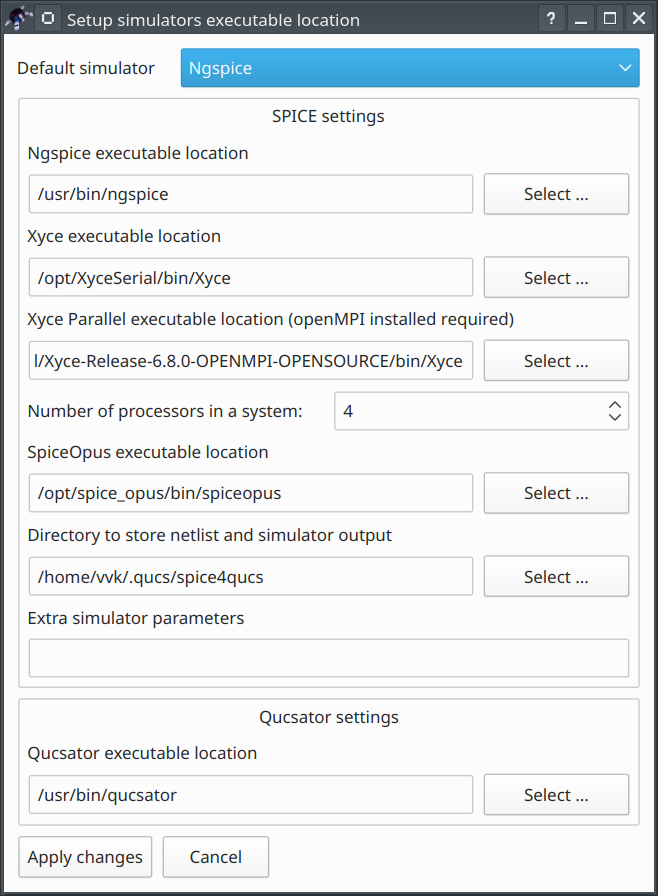
\includegraphics[width=0.4\textwidth]{sim_setup.png}
  \end{center}
  \caption{Simulator setup dialog} \label{fig:sim_setup}
\end{figure}

Quick switching of the simulation kernel without application restart is supported since version 2.0.0. See the section \ref{sec:quick_sw} for more details.

\section{Main window structure}

The Qucs-S main window is shown in the Fig. \ref{fig:mainwin}. The main window consists of two areas: schematic editor (4) on the right side and main dock (1) on the left side. Several schematics could be opened simultaneously. It's possible to switch between the opened schematics using the tabular bar above the schematic editor area.

\begin{figure}[!ht]
  \begin{center}
    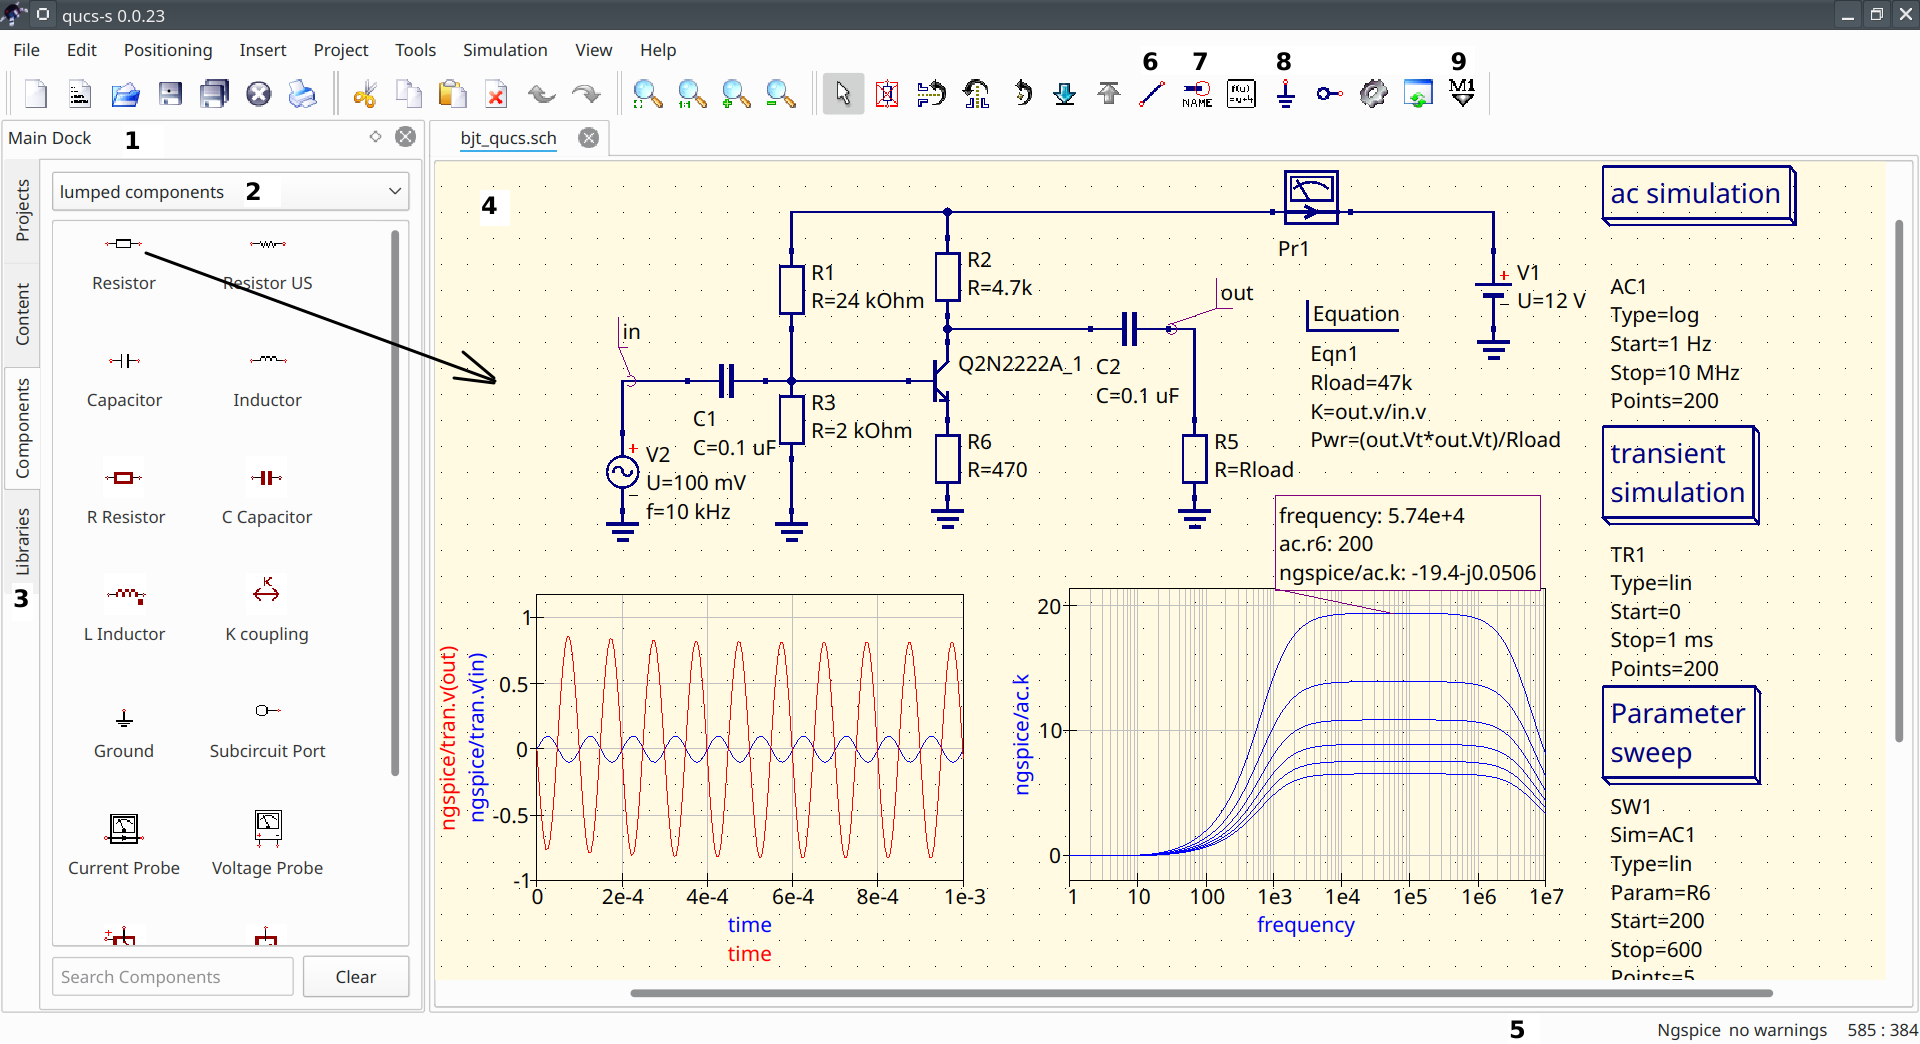
\includegraphics[width=\textwidth]{mainwin.png}
  \end{center}
  \caption{Qucs-S main window. See text for explanations} \label{fig:mainwin}
\end{figure}

The dock on the left side has four tabs (3): \emph{Projects}, \emph{Content}, \emph{Components}, and \emph{Libraries}. The \emph{Projects} tab is opened after the application start. It is empty, because there is no projects after the fresh installation. The \emph{Components} tab (see Fig. \ref{fig:mainwin}) contains a list of primitive devices available in Qucs. The components are divided into several categories (lumped devices, nonlinear devices, simulation, etc.). The categories could be selected from the drop-down list (2). The status bar is located on the bottom side of the main window. The active simulation kernel is displayed on the status bar (for example Ngspice on Fig.\ref{fig:mainwin}).

The toolbar area is located on the top side of the main window below the main menu. Some important buttons are located on the toolbar. They are: \emph{Wire} (6), \emph{Node name} (7), \emph{Ground} (8), and \emph{Marker} (9).

Everything in Qucs-S is considered to be a component. The simulations, equations, and SPICE directives are also special components that could be found in dedicated categories in the component pallet. The diagrams are also special components and could be found in the \emph{diagrams} category in the drop-down list (2).

To place the component on schematic choose desired category from the drop-down list (2) (for example "lumped components") and click on the symbol (for example "Resistor"). Moving the mouse cursor into the working area (4) you are carrying a drawing of a resistor symbol. Pressing the right mouse button rotates the symbol, pressing the left mouse button places the component onto the schematic.

The components properties could be edited using the properties dialog (Fig. \ref{fig:prop_dlg}) that is called from the context menu of the component or after the left mouse button double click.

\begin{figure}[!ht]
  \begin{center}
    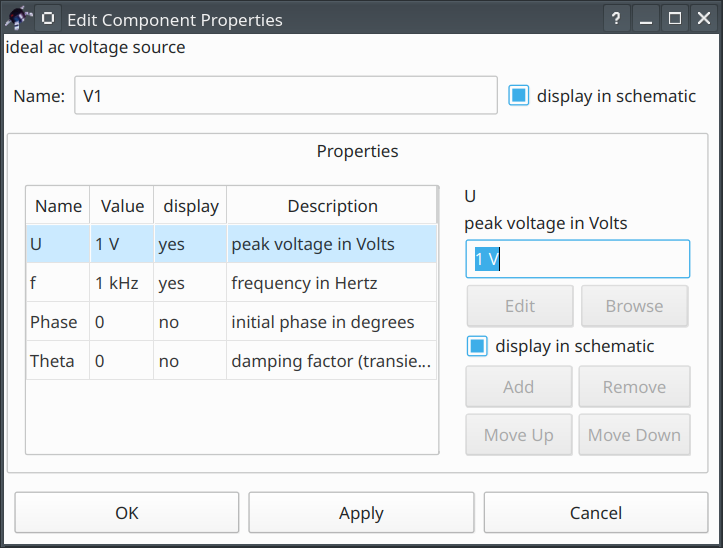
\includegraphics[width=0.45\textwidth]{prop_dlg.png}
  \end{center}
  \caption{Component properties dialog} \label{fig:prop_dlg}
\end{figure}

\section{Step by step guide how to setup an analog simulation}

\subsection{AC and transient simulation}

Let's simulated an RC-circuit using Qucs-S with Ngspice backend. The schematic is shown in the Fig. \ref{fig:rc}. Let's perform the AC and transient simulations and plot the magnitude response of the circuit and the waveforms on the input and output nodes. Perform the following steps to draw the schematic and setup the simulation.

\begin{figure}[!ht]
  \begin{center}
    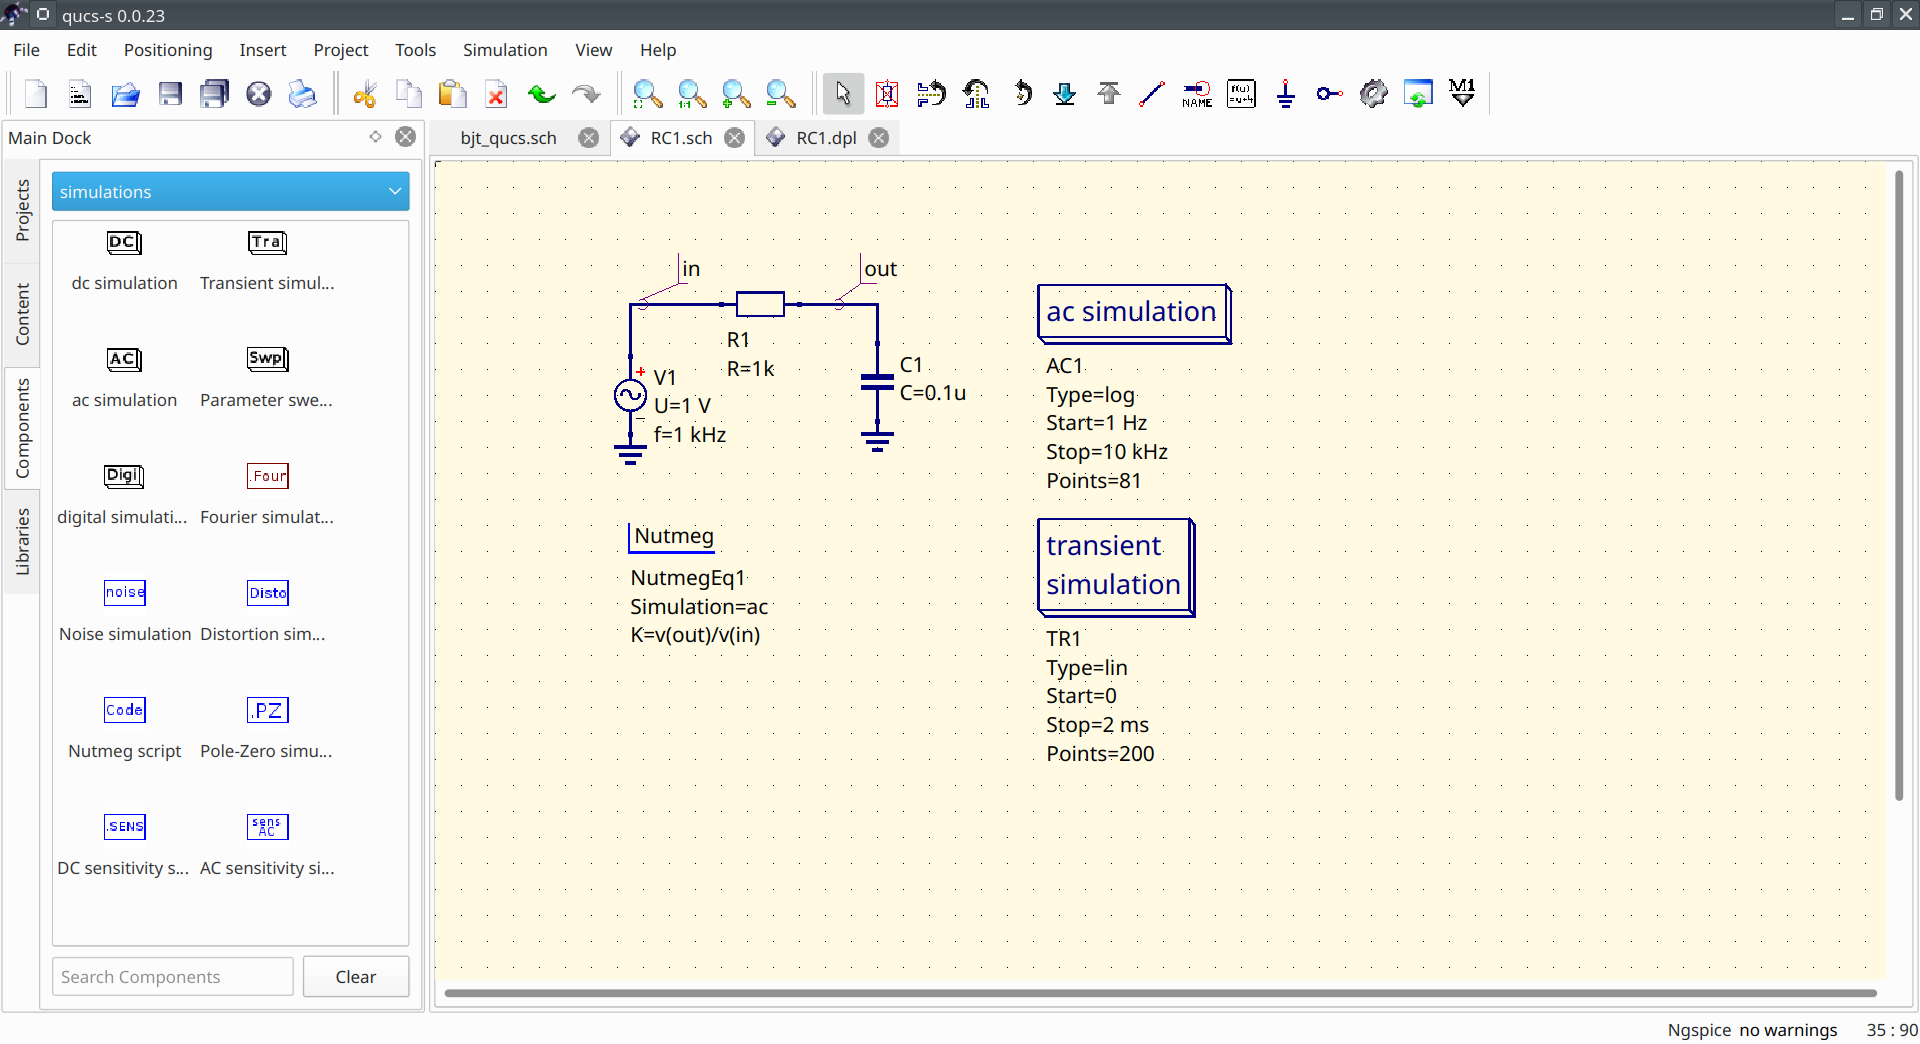
\includegraphics[width=\textwidth]{rc.png}
  \end{center}
  \caption{RC-circuit in Qucs-S} \label{fig:rc}
\end{figure}


\begin{itemize}
 \item \textbf{Step 1:} place components on the schematic and set their properties as show in the Fig. \ref{fig:rc}. We need resitor, capacitor (both could be found in the \emph{lumped devices} category) and AC voltage source (from \emph{sources} category). The ground and wires could be taken from the application tool bar (see Fig. \ref{fig:mainwin}) using the buttons (6) and (8).

 \item \textbf{Step 2:} place simulations on the schematic. We need AC simulation and Transient simulation. Both could be taken from the \emph{simulations} category (see Fig. \ref{fig:rc}). The procedure is same as for usual components. Setup the properties of the simulations as shown in the Fig. \ref{fig:rc}. A special dialog window opens upon the double click on the simulation device (Fig. \ref{fig:dlg_sim}). For AC simulation enter the start (1 Hz) and stop (10 kHz) frequencies and select the logarithmic sweep type. For transient simulation enter the stop time (2 ms) and points number (200 points).
 \begin{figure}[!ht]
  \begin{center}
    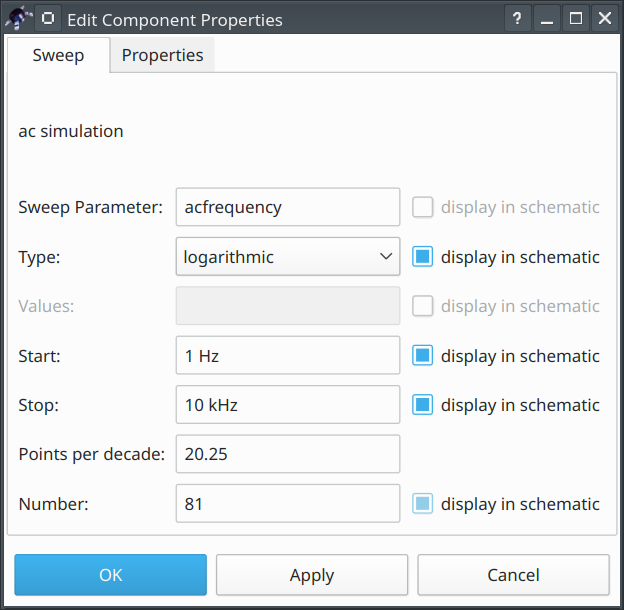
\includegraphics[width=0.45\textwidth]{dlg_sim.png}
  \end{center}
  \caption{Simulation properties dialog} \label{fig:dlg_sim}
\end{figure}

 \pagebreak[4]

 \item \textbf{Step 3:} place the node labels \verb|in| and \verb|out| using the button (6) on the toolbar (see Fig. \ref{fig:mainwin}). The node name could be set in a special dialog window (Fig. \ref{fig:nod_lbl}).
 \begin{figure}[!ht]
  \begin{center}
    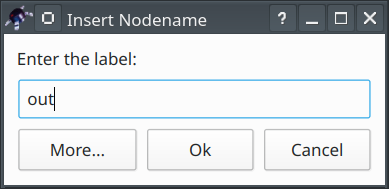
\includegraphics[width=0.4\textwidth]{nod_lbl.png}
  \end{center}
  \caption{Node label setup dialog} \label{fig:nod_lbl}
\end{figure}

 \item \textbf{Step 4:} Place equation for the magnitude response $K=V_{out}/V_{in}$ on the schematic. Equation is the special component called \emph{Nutmeg equation} that could be found in the \emph{spice specific sections} category. The full SPICE syntax for mathematical functions and node names is supported. Refer to Ngspice manual for more details. The simulation should be specified for each Nutmeg equation. We will calculate the magnitude response for the AC simulation only and therefore we need to enter \verb|ac| as the first property for this device as shown on the Fig. \ref{fig:eq}.
  \begin{figure}[!ht]
  \begin{center}
    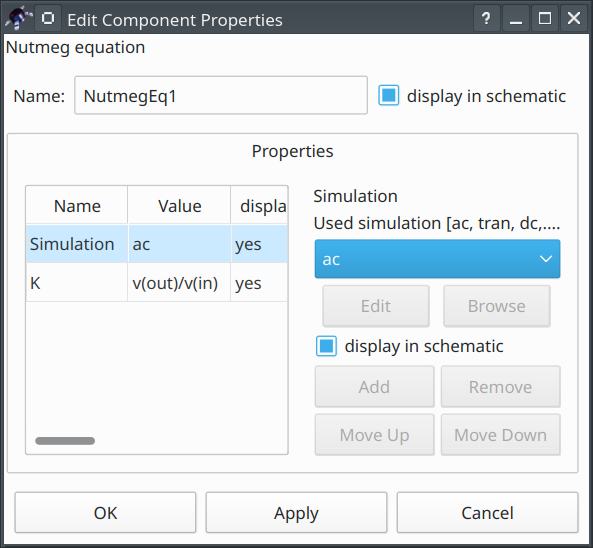
\includegraphics[width=0.4\textwidth]{nutmeg_eq.png}
  \end{center}
  \caption{Equation setup dialog} \label{fig:eq}
\end{figure}

 \item \textbf{Step 5:} Save the schematic document as the file with the \verb|*.sch| extension using the \textit{File} \verb|->| \textit{Save as} menu or press the \verb|Ctrl-S| shortcut. The schematic is ready for the simulation now.

 \item \textbf{Step 6:} simulate the schematic. Press the \textit{Simulation} \verb|->| \textit{Simulate} or press the F2 hotkey on the keyboard. The dialog window containing the simulator log messages will appear shortly (Fig. \ref{fig:sim_dlg}). This dialog window contains the simulation console where the messages from the Ngspice are shown.

 It should report that the simulation finished without errors. If you see error messages check your schematic and application settings. After the Ngspice reports about the finished simulation, close this window clicking the \emph{Exit} button. Now the diagrams could be added on schematic field. It is also possible to save the netlist file from this dialog
 .
  \begin{figure}[!ht]
  \begin{center}
    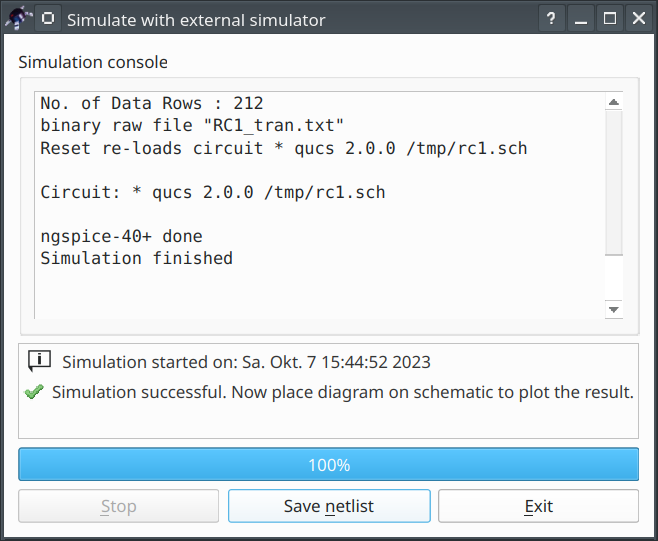
\includegraphics[width=0.4\textwidth]{sim_dlg.png}
  \end{center}
  \caption{Simulation dialog} \label{fig:sim_dlg}

\end{figure}

\item \textbf{Step 7:} place diagrams on the schematic (Fig. \ref{fig:rc_dpl}). We need two cartesian diagrams for magnitude response and transient waveforms. The diagrams are also special components that could be found in the \emph{diagrams} category. The traces could be selected in the special diagram properties dialog (Fig. \ref{fig:diagr_dlg}). Select the \verb|ac.k| traces for one diagram and \verb|tran.v(in)| and \verb|tran.v(out)| traces for another diagram. It is also possible to setup the axis limits and type and the color scheme for the diagram. Select logarithmic X-axis for the magnitude response graph using the settings in the \emph{Properties} tab. The markers could be placed on graphs using the button (9) from the toolbar (Fig. \ref{fig:mainwin}). The position of the marker could be adjiusted using the arrow keys on the keyboard.

  \begin{figure}[!ht]
  \begin{center}
    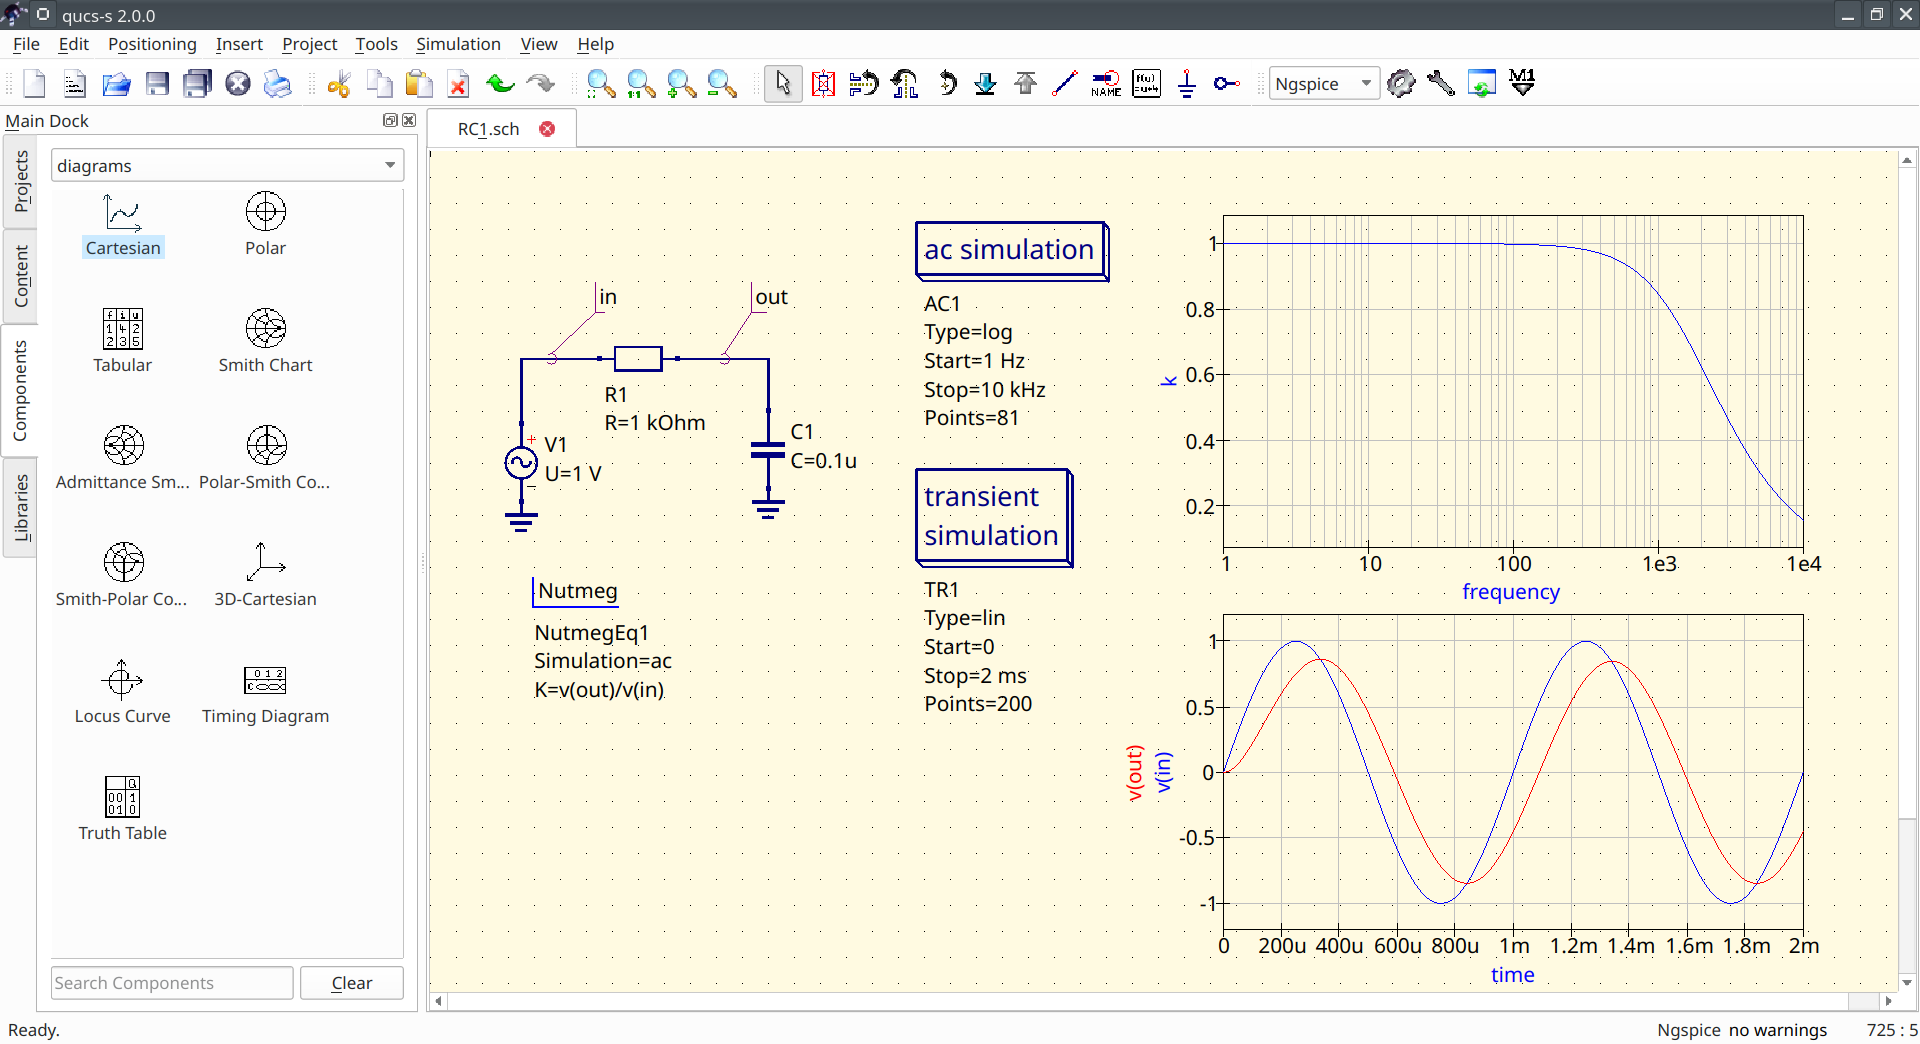
\includegraphics[width=\textwidth]{rc_dpl.png}
  \end{center}
  \caption{Schematic with two diagrams added} \label{fig:rc_dpl}
  \end{figure}

    \begin{figure}[!ht]
  \begin{center}
    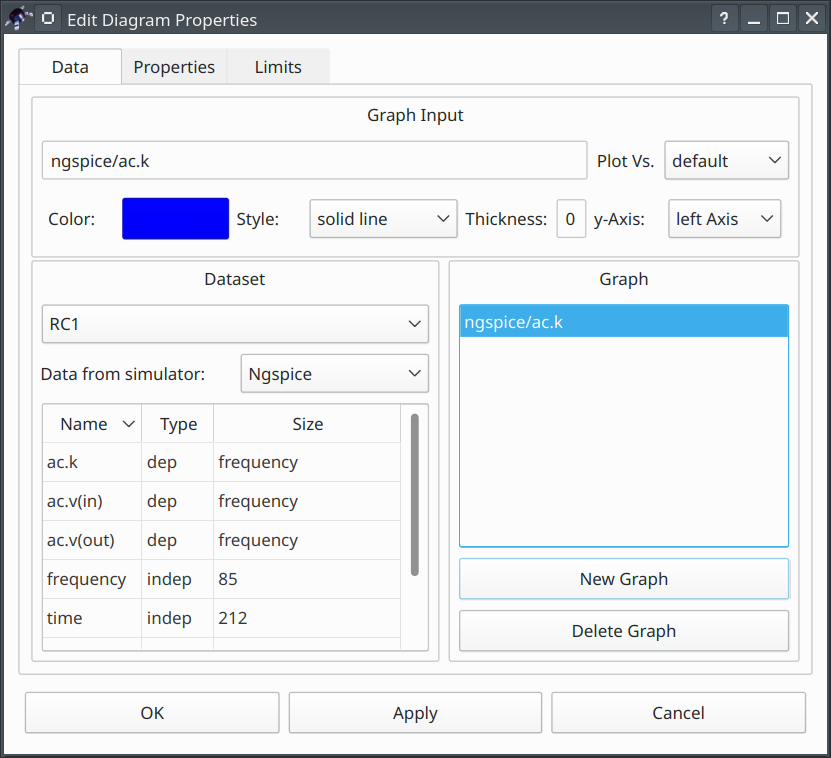
\includegraphics[width=0.4\textwidth]{diagr_dlg.png}
  \end{center}
  \caption{Diagram properties dialog} \label{fig:diagr_dlg}
  \end{figure}

\end{itemize}

\subsection{DC analysis} \label{sec:dc}

Qucs-S unlike Qucs has no special DC simulation mode. If only \emph{DC
simulation} component is placed on the schematic no simulation will be launched
and error message will be shown. This component is kept for backward
compatibility with old Qucs schematics.

But there exists two modes of the DC simulation:

\begin{itemize}
 \item Show operating point directly on the circuit. This mode is activted when
pressing F8 keyboard shortcut or using \emph{Simulation->Show bias} menu
entry. See the Fig. \ref{fig:rdiv_f8} for example of such simulation.
 \item DC sweep mode. You need to insert \emph{Parameter sweep} simulation
component and attach it to the DC simulation. This simulation mode could be
used for plotting IV-curves or getting table output. See the Fig.
\ref{fig:rdiv_dc} for example of this simulation.
\end{itemize}


\begin{figure}[!ht]
    \begin{center}
        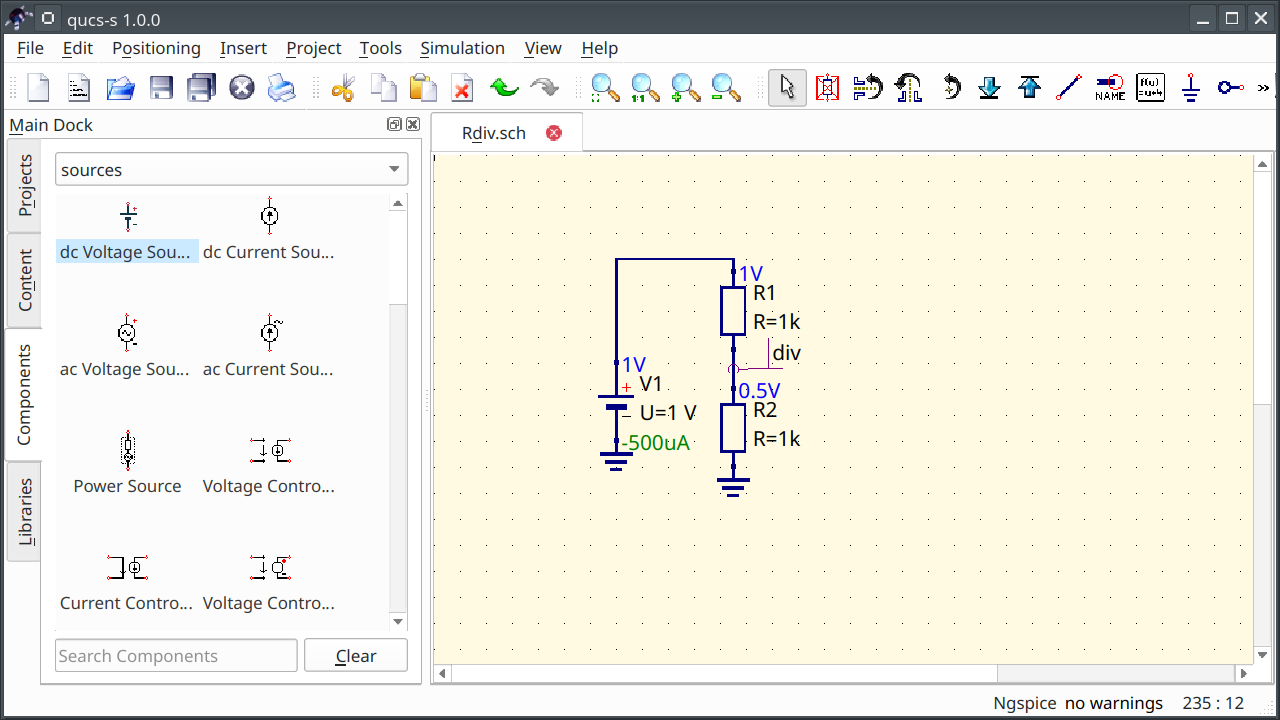
\includegraphics[width=0.8\textwidth]{rdiv_f8.png}
    \end{center}
    \caption{Operating point simulation of the voltage divider}
\label{fig:rdiv_f8}
\end{figure}


\begin{figure}[!ht]
    \begin{center}
        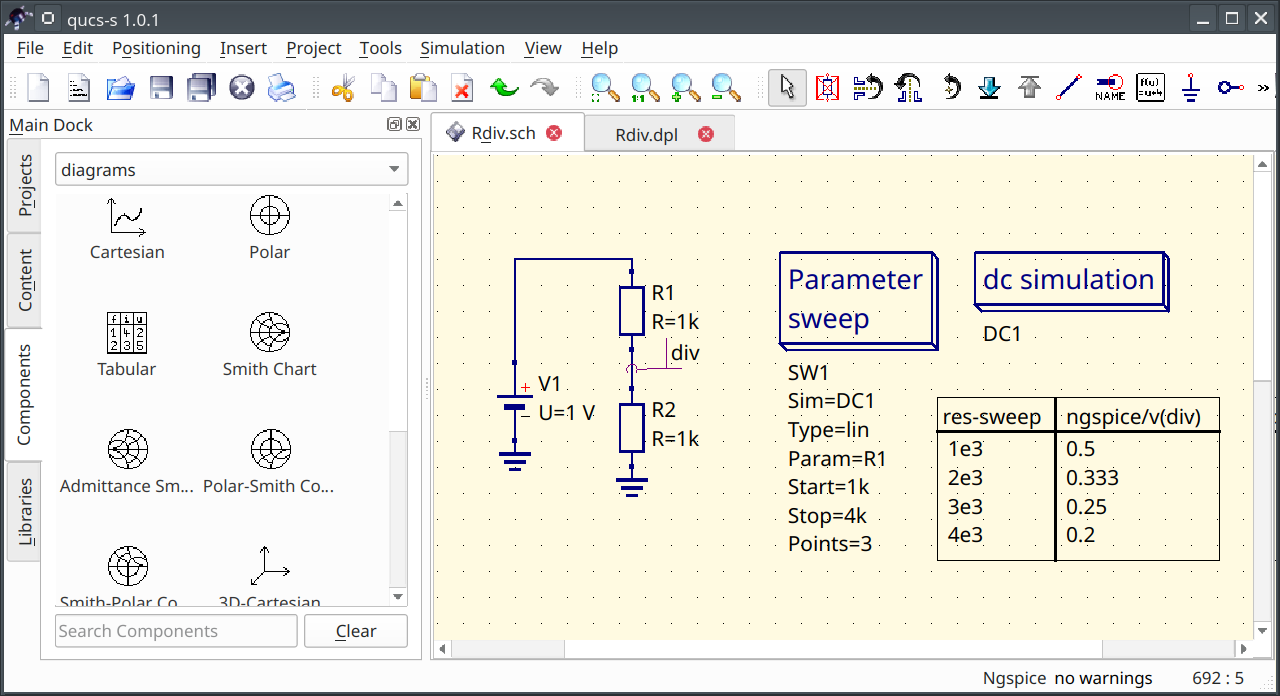
\includegraphics[width=0.8\textwidth]{rdiv_dc.png}
    \end{center}
    \caption{Using DC sweep to get table output of the resistive divider
voltage}
\label{fig:rdiv_dc}
\end{figure}

\section{Parameter sweep}

\subsection{Device sweep}

Parameter sweep is defined as the special simulation type that is attached to any other simulation. Let's consider an example
and attach parameter sweep to the circuit shown in the Figure \ref{fig:rc}. We will see the influence of the resistance of
the RC-circuit on the cutoff frequency.

\textbf{Important note:} unlike Qucs before version 0.0.20, Qucs-S doesn't support the sweep of variables directly. Legacy Qucs schematics using variable sweep will not work. Parameter sweep supports only device sweep. Resistor, capacitor or source are accepted.

Perform the following steps to add parameter sweep:

\begin{itemize}
 \item \textbf{Step 1:} Place parameter sweep component on the schematic sheet (Figure \ref{fig:rc_parsw}).
 The \emph{Parameter sweep} device could be found in the \emph{simulations} group.

    \begin{figure}[!ht]
        \begin{center}
            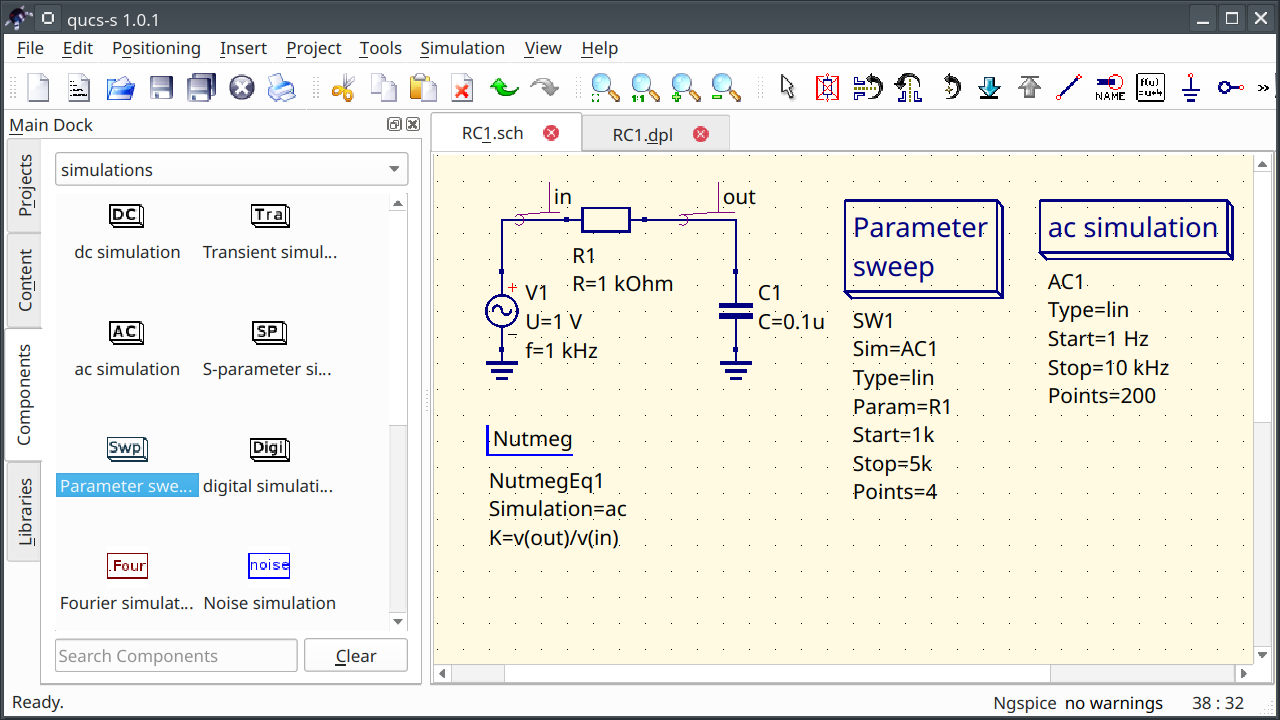
\includegraphics[width=0.8\textwidth]{rc_parsw.png}
        \end{center}
        \caption{Adding parameter sweep on the schematic}
    \label{fig:rc_parsw}
    \end{figure}

\item \textbf{Step 2:} Set the properties of the parameter sweep simulation. After the double click the dialog window will be
opened (Figure \ref{fig:parsw}). The \emph{Simulation} drop-down list is the the name of simulation component to which the parameter sweep is attached. For our example we need to select the \verb|AC1| simulation from the drop-down list, because we attaching the parameter sweep to the AC simulation. The \emph{Sweep parameter} input field is the \textbf{device} name. Variables or other objects
name are not acceptable here! Enter the \verb|R1| device name here. The \emph{Start}, \emph{Stop}, \emph{Step}, and \emph{Number} input fields serve for the definition of the sweep range. We will sweep the \verb|R1| value from 1 kOhm to 5 kOhm and take 4 sweep points.

    \begin{figure}[!ht]
        \begin{center}
            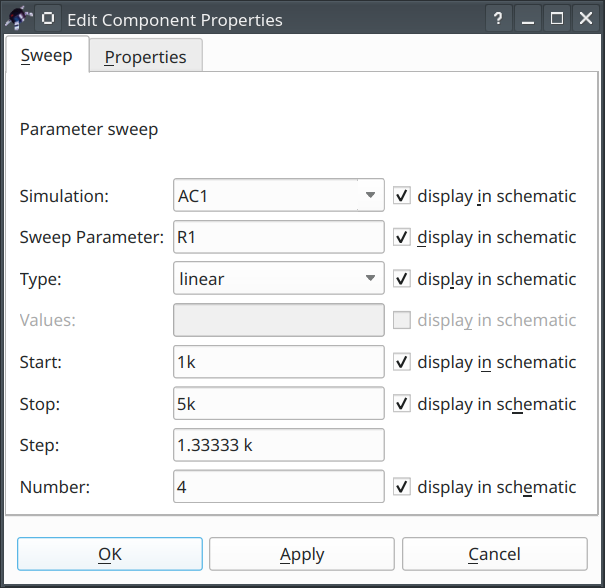
\includegraphics[width=0.5\textwidth]{parsw_dlg.png}
        \end{center}
        \caption{Setting parameter sweep properties}
    \label{fig:parsw}
    \end{figure}

\item \textbf{Step 3:} Run the simulation and place the diagrams as for usual simulation (Figure \ref{fig:parsw_mr}). You should see the family of the curves. You may place a marker on the diagram and move it between the sweep curves with \emph{Arrow Up} and \emph{Arrow Down} keys.

        \begin{figure}[!ht]
        \begin{center}
            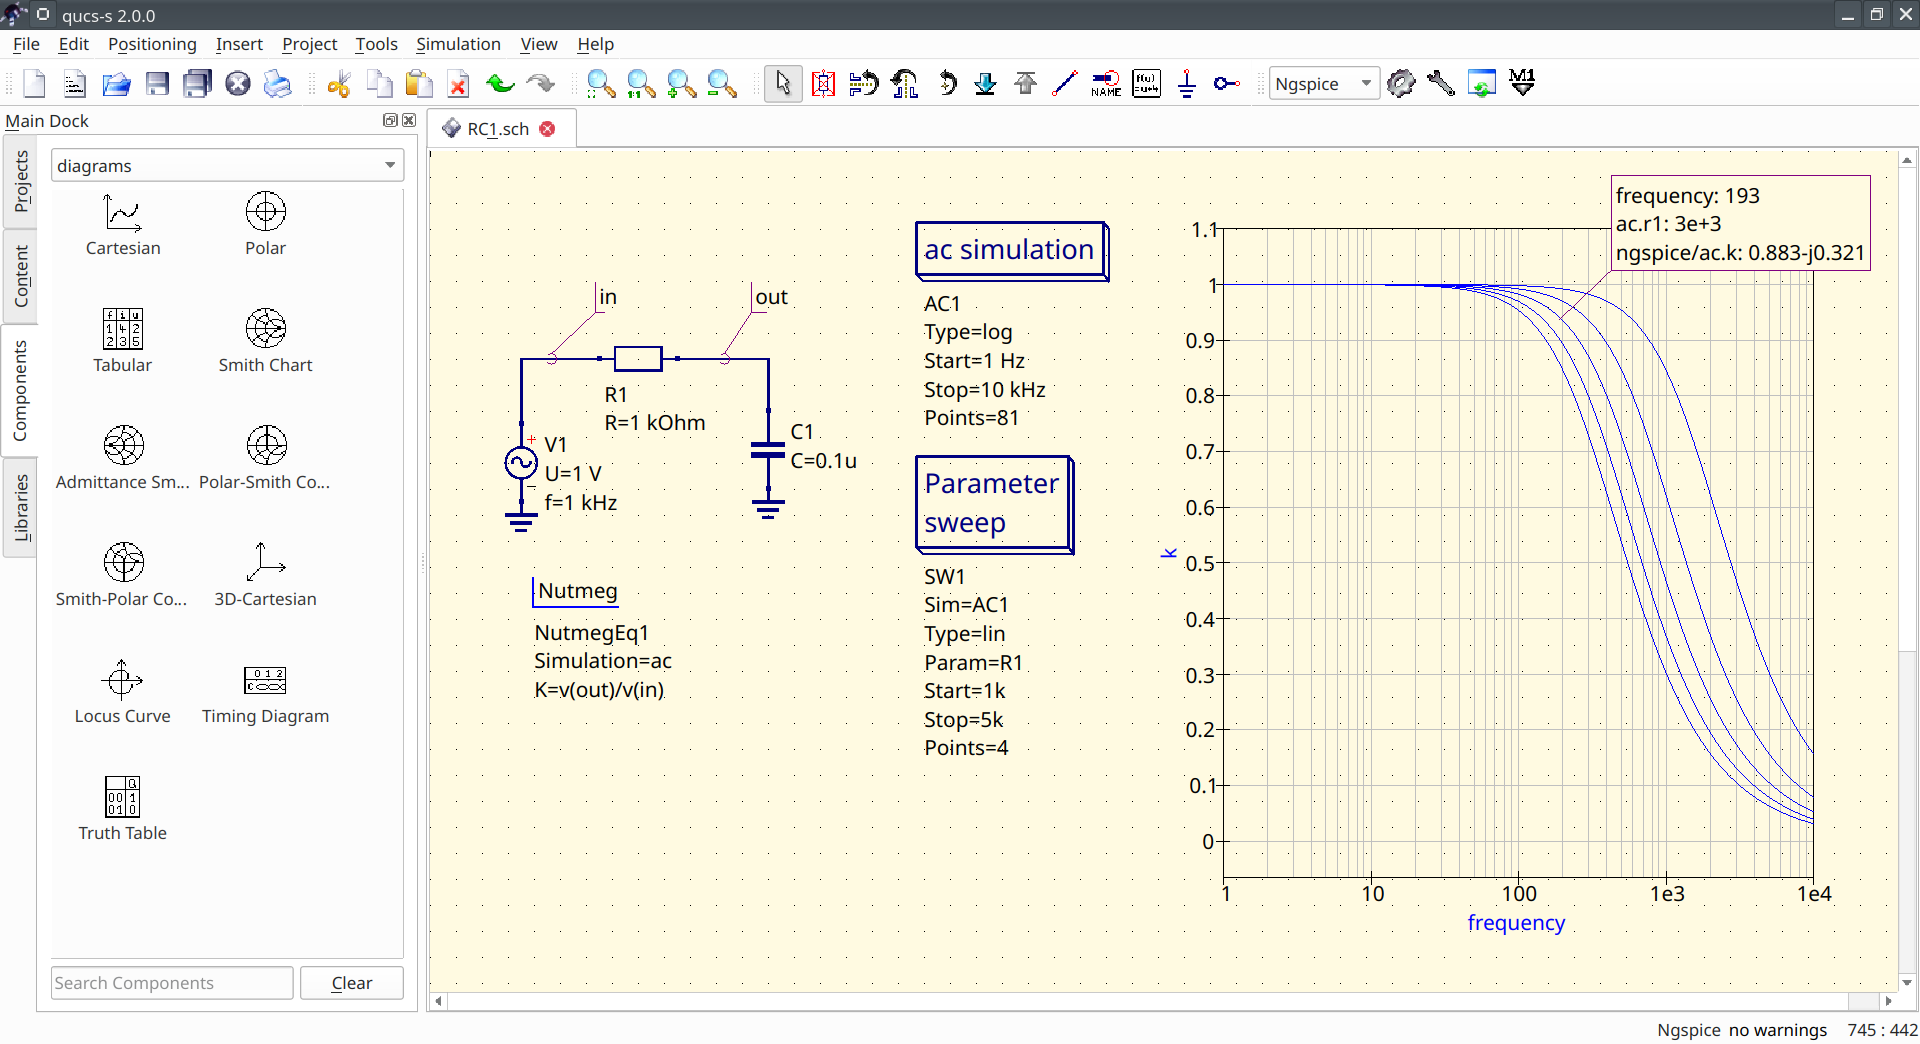
\includegraphics[width=0.8\textwidth]{parsw_mr.png}
        \end{center}
        \caption{Magnitude response of the RC-circuit with the parameter sweep}
    \label{fig:parsw_mr}
    \end{figure}

\end{itemize}


\subsection{DC sweep}

DC sweep simulation takes place when parameter sweep is attached to the DC simulation. Such simulation mode is explained in
the Section \ref{sec:dc}. DC sweep only accepts device name (resistor or source) as the sweep parameter name. The DC sweep with variable name will not work. This simulation mode usually serves for obtaining the IV-curves.

\subsection{Variable sweep}

The recent version of the Ngspice support sweeping of the varibles. The variable should be defined using the \verb|.PARAM|
statement (available at the \emph{SPICE specific sections} group). Qucs-S doesn't create the variable automatically. Refer to the schematic shown in the Figure \ref{fig:rc_parsw_var} for the example of such simulation mode.

\begin{figure}[!ht]
    \begin{center}
        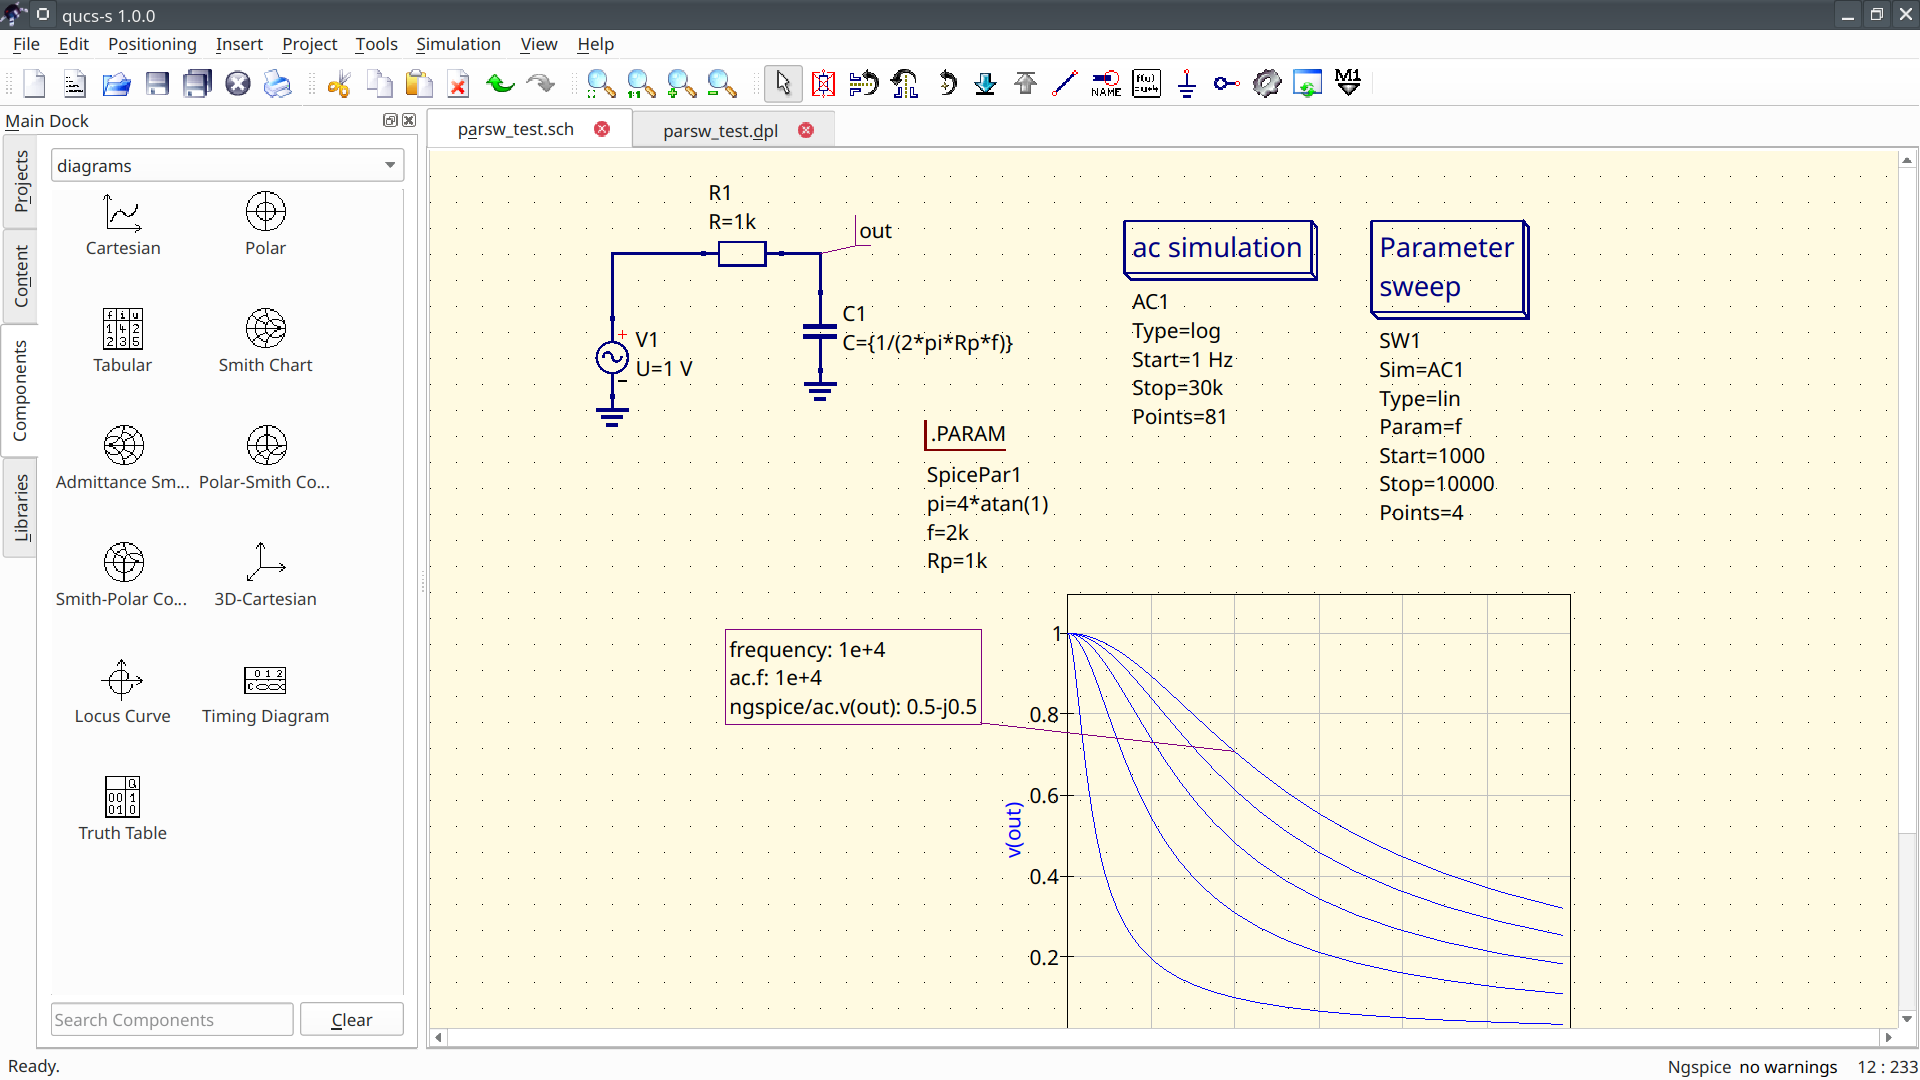
\includegraphics[width=0.8\textwidth]{rc_parsw_var.png}
    \end{center}
    \caption{Magnitude response of the RC-circuit with the parameter sweep}
    \label{fig:rc_parsw_var}
\end{figure}

\subsection{Double (nested) sweeps}

In some cases, you need to sweep two parameters, in a nested way. For example, if you want to obtain the $V_{CE}$/$I{C}$ curves of a transistor, you need to sweep the collector--emitter  voltage and, once done it, repeat for a different value of base current. In the figure~\ref{fig:double-sweep-bjt-mos} you can see how you can implement it.

\begin{figure}[!ht]
    \begin{center}
        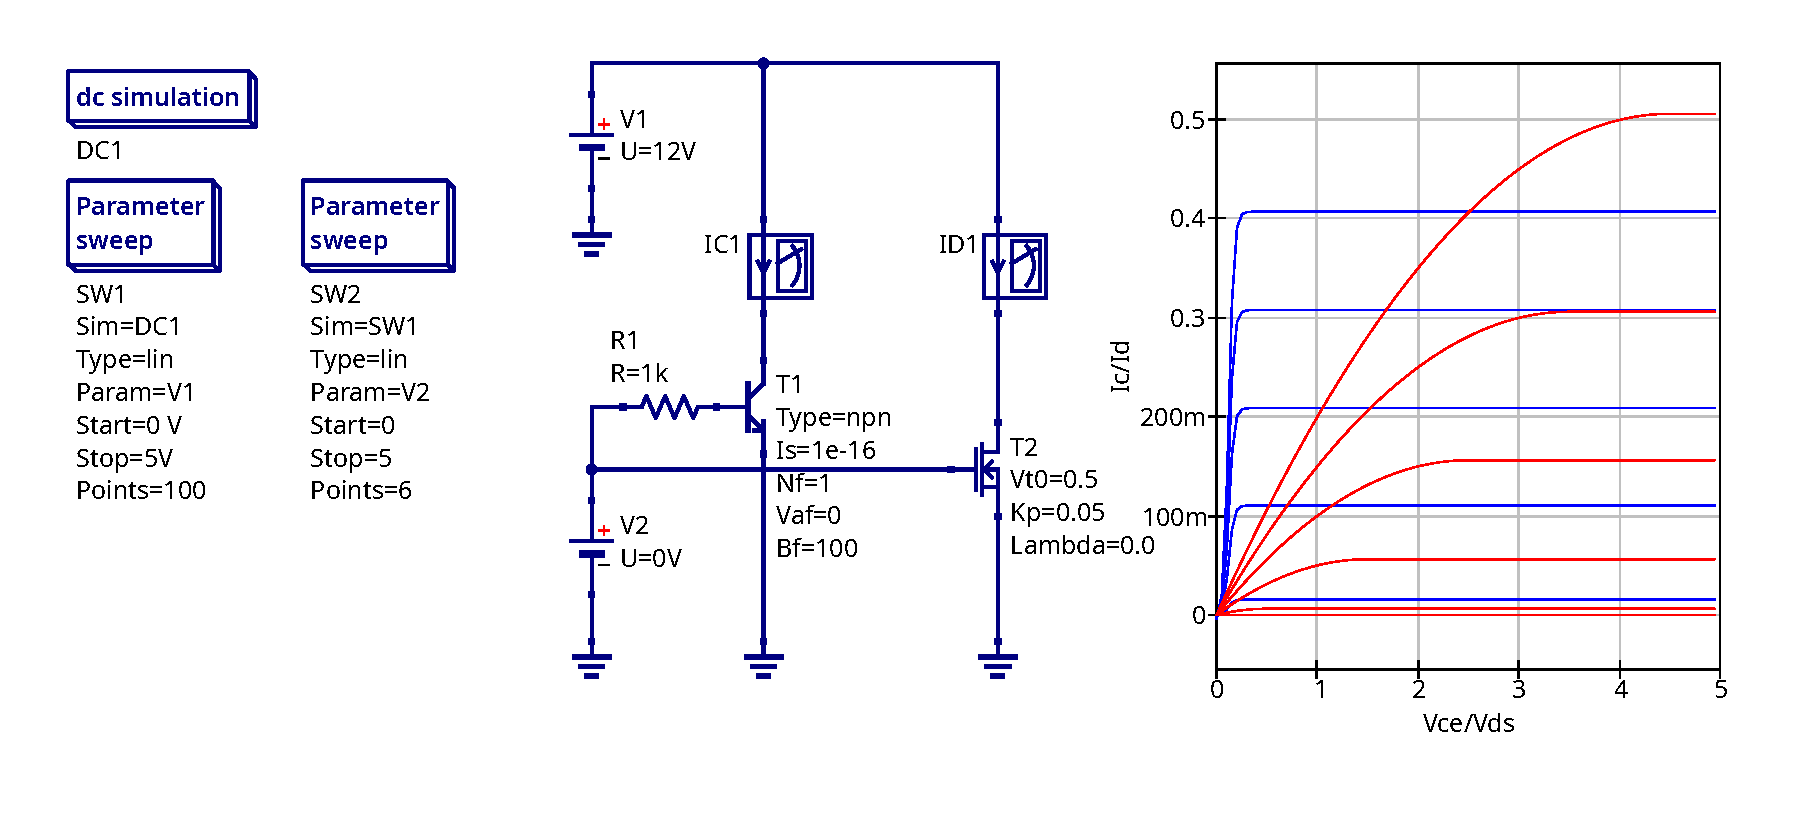
\includegraphics[width=0.8\textwidth]{double-sweep-bjt-mos}
    \end{center}
    \caption{Comparing the characteristics of BJT and MOSFET with two nested sweeps}
    \label{fig:double-sweep-bjt-mos}
\end{figure}

The trick is to first add a parameter sweep, that act on a simulation, exactly as before:
as you can see, the parameter sweep \texttt{SW1} acts on the \texttt{DC1} simulation. After that, you add another parameter sweep ``block'' that acts \emph{on the previous sweep}: notice how the \texttt{SW2} parameter sweep has \texttt{Sim=SW1}.

After running the simulation, you can plot for example the two currents, which in this case are called \texttt{sw1.i(vic1)} y \texttt{sw1.i(vid1)}, and depends on the rather strange \texttt{sw1.v(v-sweep) sw1.v2}.

\section{Digital simulation}

\subsection{Digital devices with analog model}

Digital devices including logic gates, flip-flops, and more complex devices could be found in the group \emph{Digital components}. Some of these devices have both analog and digital model. Ngspice simulation operates using XSPICE models. Here is the list of these devices:

\begin{itemize}
 \item Logic gates, inverter and buffer
 \item D-, JK-, T-flip-flops
 \item Digital source
\end{itemize}

The usage of these devices in analog simulation mode has no special requirements. The example shown in the Figure \ref{fig:logic_gen} illustrates the transient simulation of the RC oscillator circuit containing two inverter logic gates. The power supply voltage for digital devices should be set using the \verb|VCC| parameter with \verb|.PARAM| section.

    \begin{figure}[!ht]
    \begin{center}
        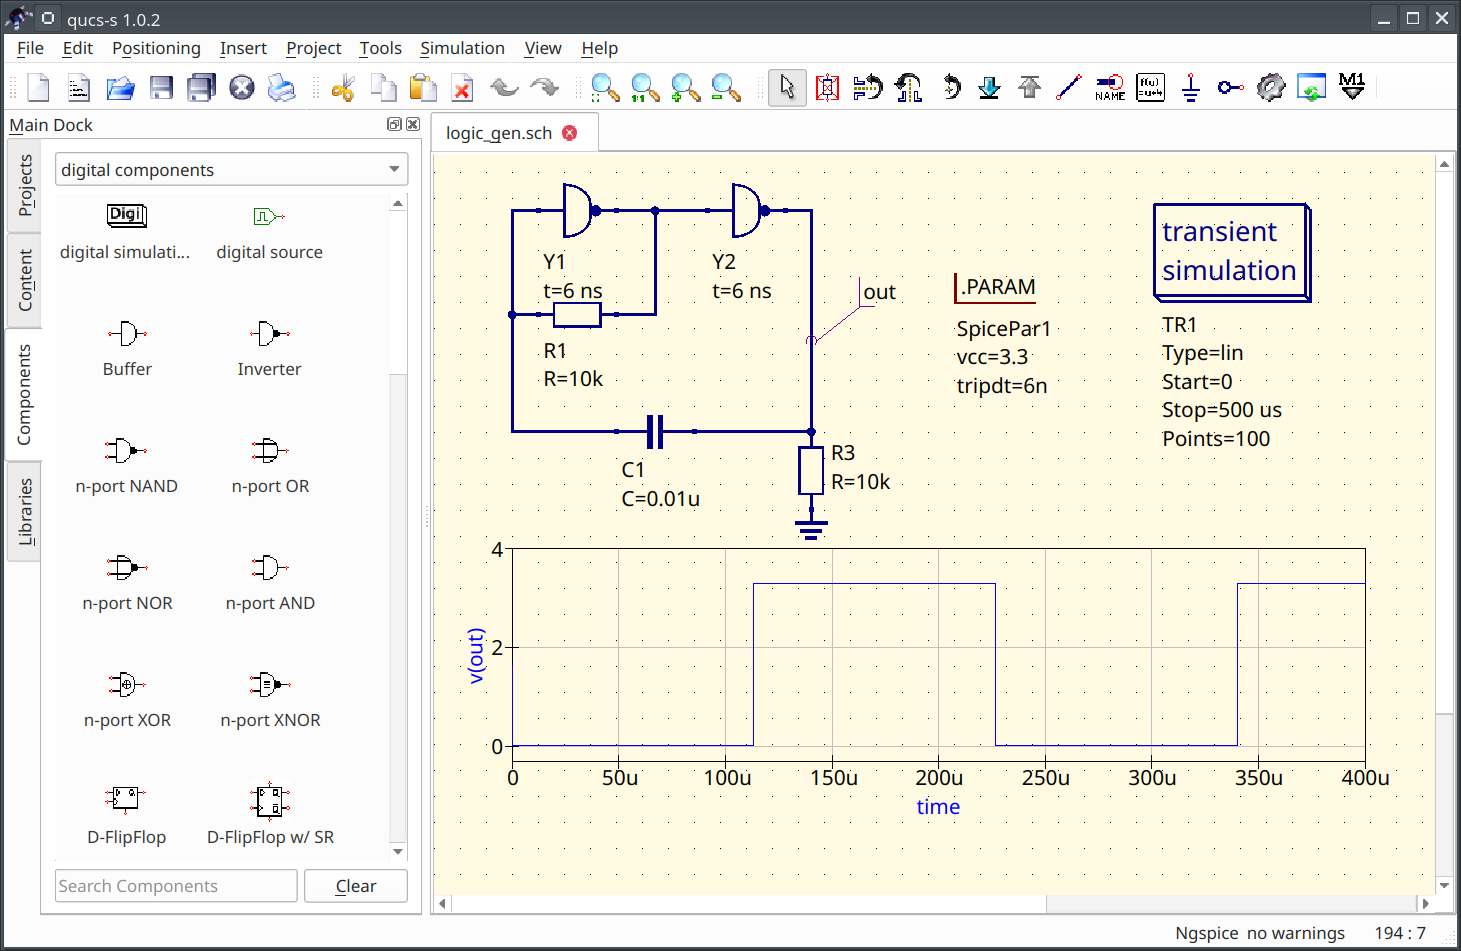
\includegraphics[width=0.8\textwidth]{logic_gen.png}
    \end{center}
    \caption{Oscillator example using logic gates} \label{fig:logic_gen}
    \end{figure}


\subsection{Digital simulation with Verilog/VHDL} \label{sec:digi}

The most of digital components except of the listed in the previous section doesn't contain analog SPICE model. These devices are  supported by digital simulation mode only. \textbf{Mixing digital and analog devices (like RCL) in one circuit is not supported!} You need to install one the following free backends to perform digital simulation

\begin{itemize}
 \item Icarus Verilog \verb|iverilog| \url{https://steveicarus.github.io/iverilog/}
 \item FreeHDL \url{http://freehdl.seul.org/}
\end{itemize}


Place on the schematic field a special device named \emph{Digital simulation} to switch Qucs-S to digital mode. Verilog or VHDL backend will be started automatically instead of SPICE if digital simulation is found in the schematic. User doesn't need to switch
Qucs-S to the digital mode in the application settings.

There are two modes of the digital simulation: truth table and timing diagram. An example of the digital simulation of the 2-bit decoder/demultiplexer is shown in the Figure \ref{fig:demux}. This simulation uses Verilog and timing diagram mode.

    \begin{figure}[!ht]
    \begin{center}
        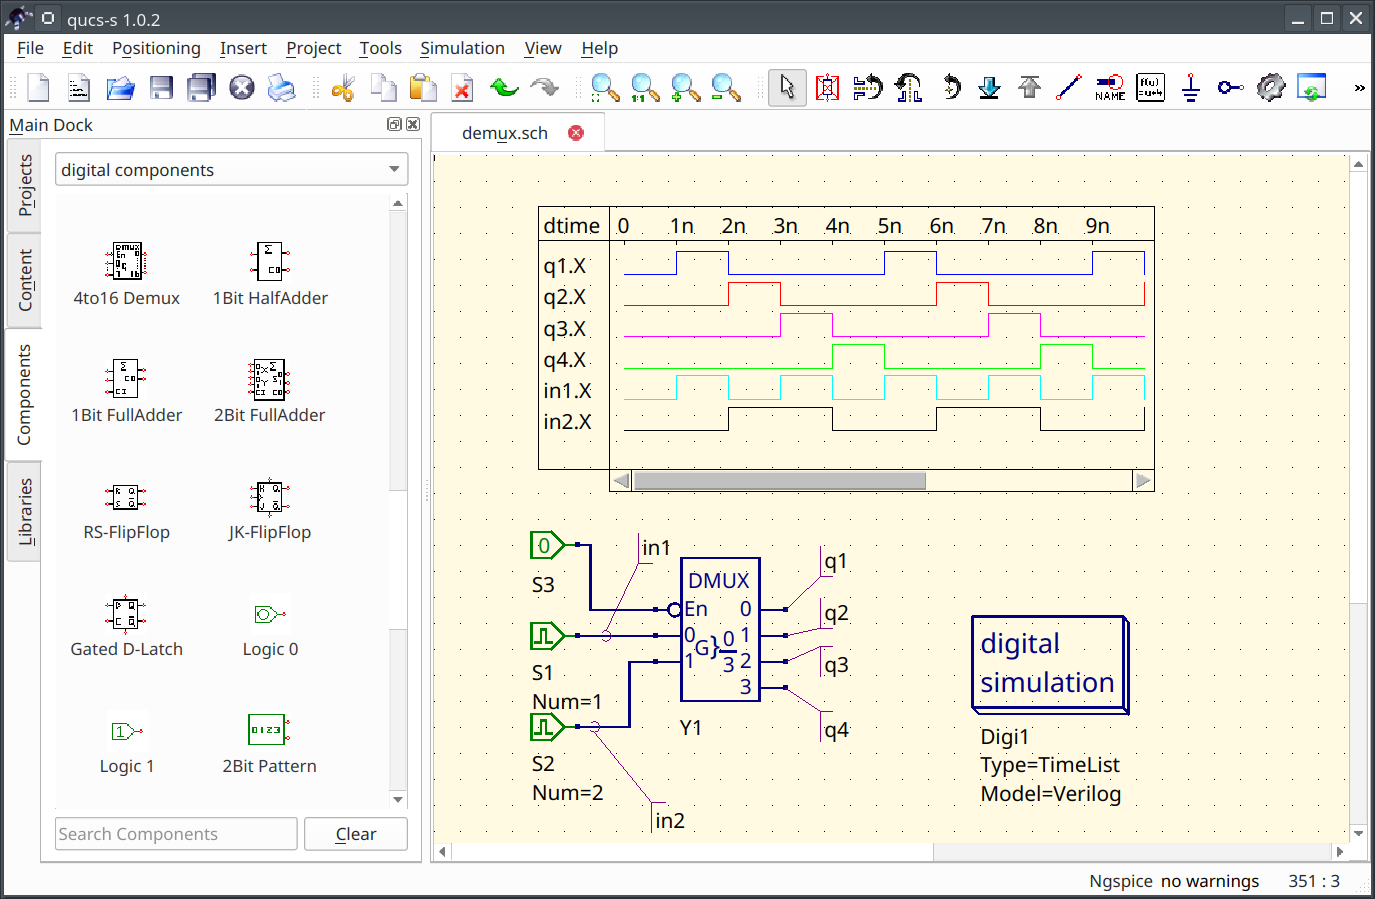
\includegraphics[width=0.8\textwidth]{demux.png}
    \end{center}
    \caption{Simulation of the digital circuit with iverilog} \label{fig:demux}
    \end{figure}


\section{Tuning mode}

Since the version v2.1.0 Qucs-S support the tuning simulation mode. The tuner allows to adjust the component property values using an interactive sliders and immediately see the result on diagrams. Tuning mode is supported for all simulation kernels including Ngspice and Qucsator. Tuner may act as an interactive alternative of the parameter sweep simulation.

Let's consider how to use the tuning mode for the RC-circuit Fig. \ref{fig:rc}. The schematic is required to have the simulations and diagrams placed on schematic. The tuner will not work without defined simulations and diagrams. The tuner is activated using the \emph{Simulation->Tune} menu or F3 keyboard shortcut. The following dialog window (Fig. \ref{fig:tuner_dlg}) is shown after the activation. Then user need to click on the device or the device property with the left mouse button. A new slider will be added to the tuner window. It is possible to manually set the upper and lower limit of the tuned device property. The default limits are within the $\pm15\%$ range from the starting value.



    \begin{figure}[!ht]
    \begin{center}
        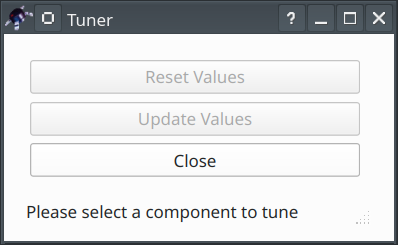
\includegraphics[width=0.3\textwidth]{tuner_dlg.png}
    \end{center}
    \caption{Tuner dialog window} \label{fig:tuner_dlg}
    \end{figure}

After the sliders are added to the tuner window it is possible to drag the sliders and observe the changes on the diagrams. For example we can see the cutoff frequency of the RC-circuit is increasing when C is decreasing. If the tuner window is closed the user will be prompted to update or revert the components values on schematic.

    \begin{figure}[!ht]
    \begin{center}
        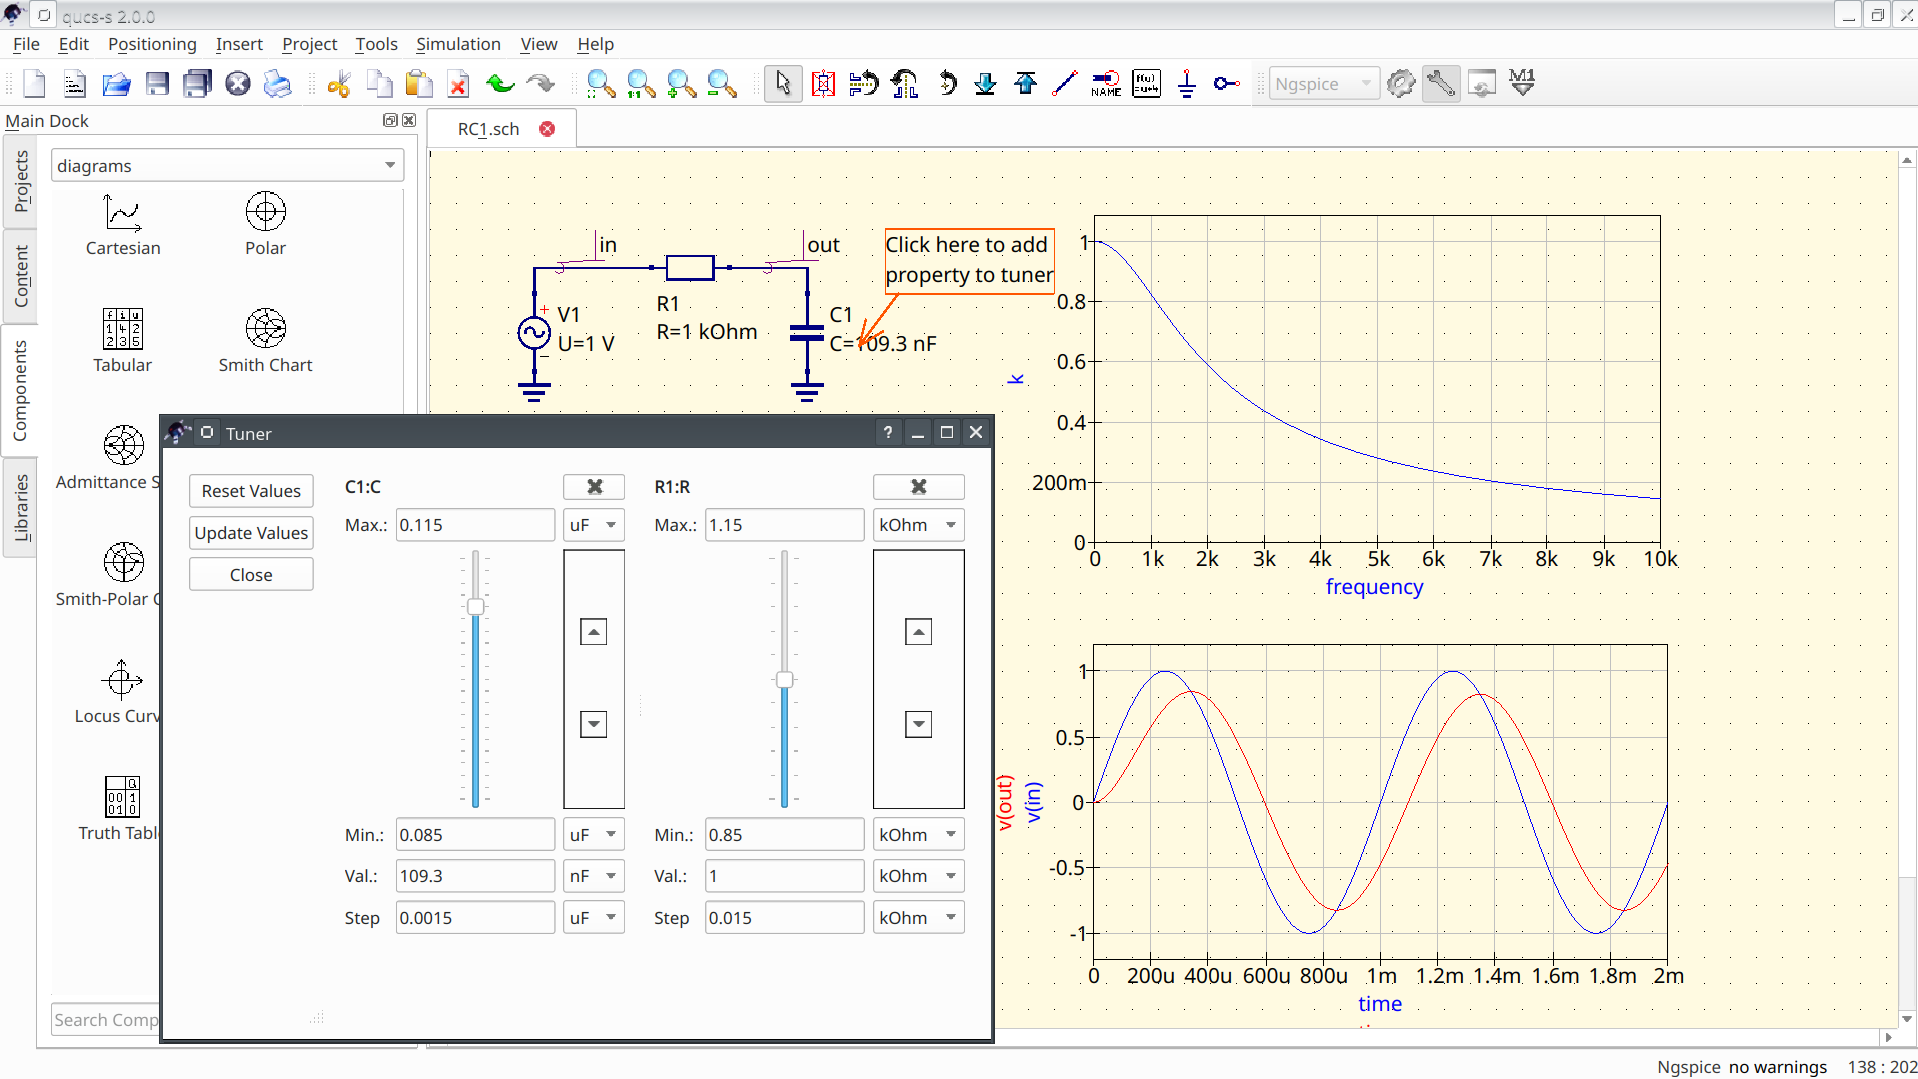
\includegraphics[width=\textwidth]{tuner_rc.png}
    \end{center}
    \caption{Tuning of the RC-circuit} \label{fig:tuner_rc}
    \end{figure}


\section{SPICE models usage}

\subsection{Importing SPICE modelcards}

The nonlinear devices models like discrete transistors and diodes are distributed as SPICE modelcards. Here is an example of the modelcard for 1N4007 diode. This modelcard defines the model named \verb|DI_1N4007|. The modelcard always starts from the \verb|.MODEL| directive.

\begin{verbatim}
.MODEL DI_1N4007 D  ( IS=76.9p RS=42.0m BV=1.00k IBV=5.00u
+ CJO=26.5p  M=0.333 N=1.45 TT=4.32u )
\end{verbatim}

Since the version 24.3.0 Qucs-S is able to fill the properties of the unified nonlinear devices from the SPICE modelcards. The following components support this feature:

\begin{itemize}
 \item Diode
 \item Bipolar transistors (NPN, PNP)
 \item MOSFETs both 3-pin and 4-pin (NMOS, PMOS)
 \item JFETs
\end{itemize}

The devices mentioned above could be found in group \emph{nonlinear components} in the left panel and have blue color. The similar red devices from \emph{microelectronics} group don't support this feature. Place the nonlinear device on schematic sheet and open device properties dialog after the double click on device or using the right mouse button click menu. The device properties dialog window has the button named \emph{Fill from SPICE .MODEL}. Press this button to import the SPICE modelcard. The following dialog window (Figure \ref{fig:spice_import}) appears. Insert the SPICE code of the modelcard in the large input filed and press OK button. The Qucs-S will recognize the SPICE model and update the device properties automatically.



    \begin{figure}[!ht]
    \begin{center}
        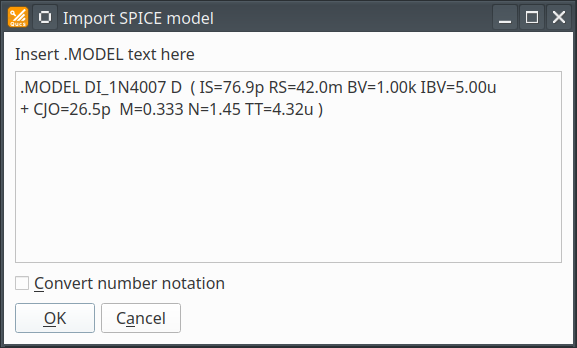
\includegraphics[width=0.4\textwidth]{import_modelcard.png}
    \end{center}
    \caption{Importing SPICE diode modelcard} \label{fig:spice_import}
    \end{figure}

The \emph{Convert number notation} checkbox enables numbers conversion to Qucs-S compatible form. Subcircuit type SPICE models cannot be imported this way.

\subsection{Importing SPICE subcircuit devices}

Complex semiconductor devices like analog and digital ICs are defined as SPICE subcircuit models. This model starts with \verb|.SUBCKT| directive. The listing below shows an example of such model for LM358 operational amplifier. Subcircuits are often collected in SPICE libraries.

\begin{verbatim}
*LM358 DUAL OPERATIONAL AMPLIFIER MACRO-MODEL
* connections:      non-inverting input
*                   |   inverting input
*                   |   |   positive power supply
*                   |   |   |   negative power supply
*                   |   |   |   |   output
*                   |   |   |   |   |
.SUBCKT LM358       1   2  99  50  28
****************INPUT STAGE**************
IOS 2 1 5N
*^Input offset current
R1 1 3 500K
R2 3 2 500K
I1 99 4 100U
R3 5 50 517
R4 6 50 517
Q1 5 2 4 QX
Q2 6 7 4 QX
*Fp2=1.2 MHz
C4 5 6 128.27P
***********COMMON MODE EFFECT***********
I2 99 50 75U
*^Quiescent supply current
EOS 7 1 POLY(1) 16 49 2E-3 1
*Input offset voltage.^
R8 99 49 60K
R9 49 50 60K
*********OUTPUT VOLTAGE LIMITING********
V2 99 8 1.63
D1 9 8 DX
D2 10 9 DX
V3 10 50 .635
**************SECOND STAGE**************
EH 99 98 99 49 1
G1 98 9 POLY(1) 5 6 0 9.8772E-4 0 .3459
*Fp1=7.86 Hz
R5 98 9 101.2433MEG
C3 98 9 200P
***************POLE STAGE***************
*Fp=2 MHz
G3 98 15 9 49 1E-6
R12 98 15 1MEG
C5 98 15 7.9577E-14
*********COMMON-MODE ZERO STAGE*********
*Fpcm=10 KHz
G4 98 16 3 49 5.6234E-8
L2 98 17 15.9M
R13 17 16 1K
**************OUTPUT STAGE**************
F6 50 99 POLY(1) V6 300U 1
E1 99 23 99 15 1
R16 24 23 17.5
D5 26 24 DX
V6 26 22 .63V
R17 23 25 17.5
D6 25 27 DX
V7 22 27 .63V
V5 22 21 0.27V
D4 21 15 DX
V4 20 22 0.27V
D3 15 20 DX
L3 22 28 500P
RL3 22 28 100K

.MODEL DX D(IS=1E-15)
.MODEL QX PNP(BF=1.111E3)

.ENDS
\end{verbatim}

Qucs-S provides a special \emph{Spice library device} component to use SPICE subcircuits in schematics. This component could be found at the \emph{File components} group in the left panel. Place the \emph{Spice library device} and enter its properties with the double click or context menu. The following dialog window (Figure \ref{fig:splibcomp}) will be opened.


    \begin{figure}[!ht]
    \begin{center}
        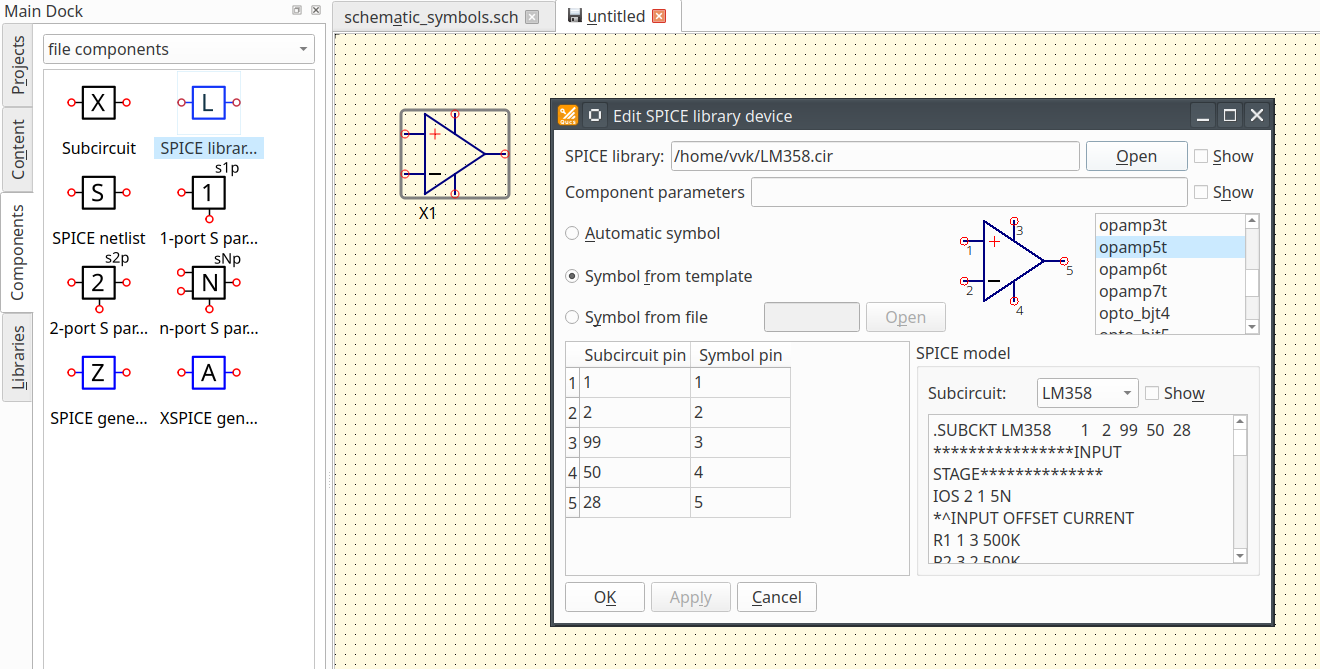
\includegraphics[width=0.9\textwidth]{splibcomp.png}
    \end{center}
    \caption{SPICE library device properties} \label{fig:splibcomp}
    \end{figure}

This dialog has a number of input fields and other input controls. Perform the following steps to setup the SPICE device properties.

\begin{enumerate}
 \item Specify the path to SPICE library file containing the subcircuit type model using the \emph{SPICE library} input field;
 \item Select SPICE model to use from the \emph{Subcircuit} drop-down list. The Qucs-S parses the specified library file and fills all found \verb|.SUBCKT| entries in this drop-down list.
 \item Select symbol for the SPICE device. Three options are available. Automatic symbol creates a rectangular symbol. Symbol from template could be selected from the list in the right side of the dialog window. The Qucs-S contains a set of symbol templates for the most common ICs and discrete devices. Also you can draw a user symbol and specify it using the \emph{Symbol from file} option. The symbol file should be saved as \verb|*.sym| and could be created using \emph{File->New symbol} in main menu.
 \item Assign symbol pin to every subcircuit pin using the table in the left part of the dialog window. The \verb|NC| in the table cells indicates that the pins are not assigned yet. All device pins must be assigned. The symbol preview in the right part of the window shows the symbol pins numbers.
\end{enumerate}

After the device and symbol are selected and pins are assigned press the OK button. The \emph{Spice Library Device} is ready for the simulation. Please keep in mind that Qucs-S doesn't embed the SPICE code in the schematic and this file device is still referencing the SPICE library file. You have to distribute the SPICE library with the schematic. Some SPICE models distributed by IC vendors may require Ngspice compatibility options setting like PSPICE/LTspice compatibility. Refer to the model description before using with Qucs-S.

\section{RF simulation}

\subsection{Common notes on RF circuits analysis}

RF circuits are often described by the scattering matrix (S-parameters). Many electrical properties of networks of components (inductors, capacitors, resistors) may be expressed using S-parameters, such as gain, return loss, voltage standing wave ratio (VSWR), reflection coefficient and amplifier stability. It is possible to convert the S-parameters to the Y or Z-matrix to estimate the input and output impedances of the circuit.

The S-parameters of the two-port circuit have the following meaning:

\begin{itemize}
 \item $S_{11}=\Gamma_1$ input reflection coefficient; if $S_{11}=0$ the circuit is ideally matched without reflection;
 \item $S_{21}$ forward power gain $G_p$ from input (port 1) to output (port 2). For passive circuits always $G_p<1$;
 \item $S_{12}$ reverse power gain from output to input.
 \item $S_{22}=\Gamma_2$ output reflection coefficient;
\end{itemize}

The VSWR and reflection coefficients are related as the following:

\begin{equation}
 \mathrm{VSWR} = \frac{1+|\Gamma|}{1-|\Gamma|}
\end{equation}

\subsection{RF simulation with Ngspice}

Ngspice supports the S-parameter simulation since the version 37. Make sure that your Ngspice package has the version above 37. Otherwise this simulation mode will not work. There exists a special S-parameter simulation component that should be placed on schematic. The input and output ports of the circuit are represented by \emph{power source} component (Fig. \ref{fig:port50}).

    \begin{figure}[!ht]
    \begin{center}
        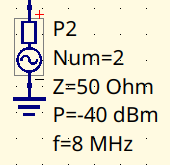
\includegraphics[width=0.2\textwidth]{port50.png}
    \end{center}
    \caption{The power source representing 50-ohm port} \label{fig:port50}
    \end{figure}

The parameters of this device are port number \verb|Num|, frequency $f$, and source power $P$ expressed in dBm. Two such sources should be connected to schematic input and output nodes respectively.

Let's consider an example and simulate the frequency response of the bandpass filter for the 20m hamradio band. The schematic is shown in the Fig. \ref{fig:filt20m}.

    \begin{figure}[!ht]
    \begin{center}
        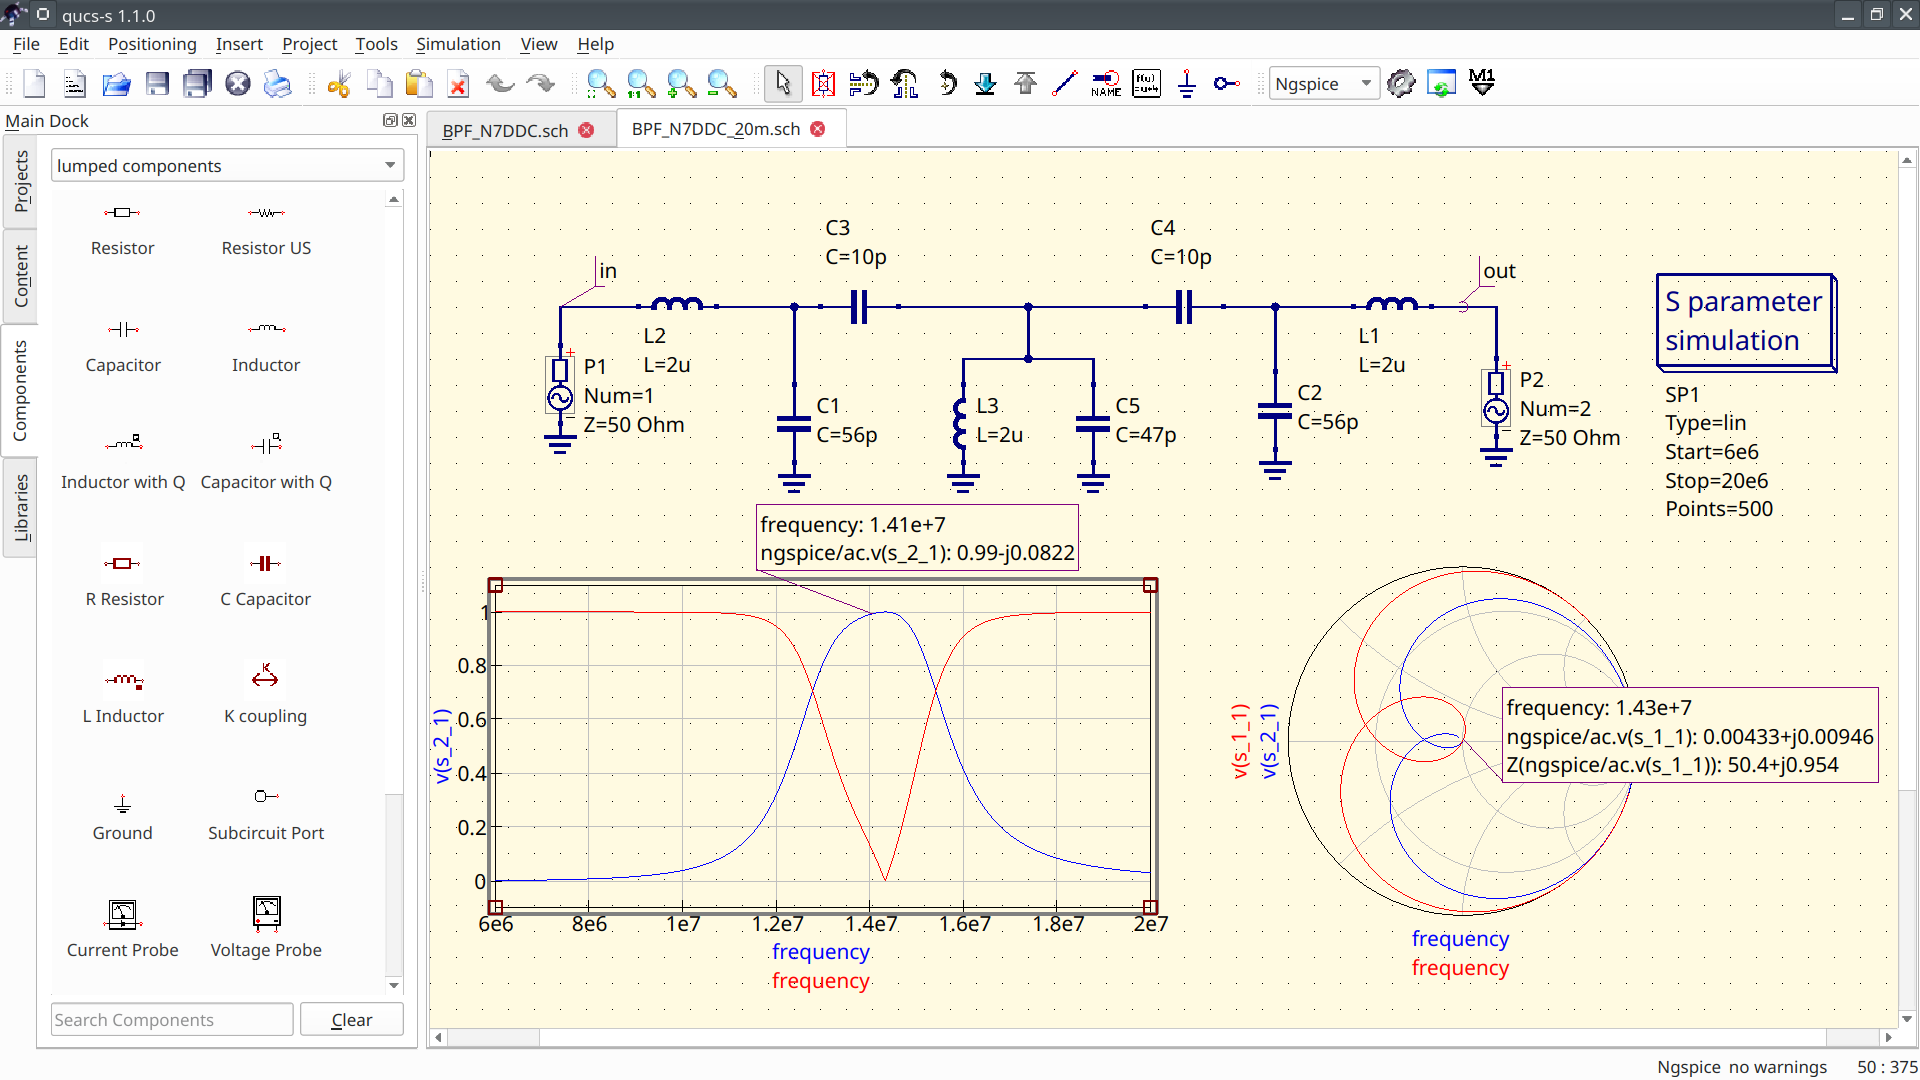
\includegraphics[width=\textwidth]{filt20sim.png}
    \end{center}
    \caption{The simulation of the band-pass filter with Qucs-S and Ngspice} \label{fig:filt20m}
    \end{figure}

The filter consists of LC-devices that could be found in the \emph{lumped devices} group. The filter schematic contains two 50-ohm port sources connected to its input and output nodes (\verb|in| and \verb|out|). The \emph{S-parameter simulation} component defines the frequency sweep range from 6 MHz to 20 MHz.

The simulation of the filter circuit could be launched as usual using the F2 keyboard shortcut. After the simulation has been finished a number of diagrams could be placed on schematic. Ngspice represents the S-parameter simulation data as the virtual voltages.For example, it's need to pick the \verb|v(s_2_1)| variable to plot the $S_{21}$ dependency. The cartesian diagram contains the $S_{11}$ and $S_{21}$ dependencies. The $S_{21}$ is the magnitude response of the filter. The same dependencies could plot on a Smith chart. Qucs-S provides a number of diagrams that could be used for RF circuits analysis. These diagrams are: Smith chart, admittance Smith chart, polar complex plane, and combined Smith chart and complex plane.

Ngspice converts the S-matrix to Y- and Z-matrix automatically. The Y and Z-parameters frequency dependencies could be plotted after the simulation. The Y and Z parameters are slow represented as the virtual voltages by Ngspice. For example the \verb|v(z_1_1)| variable will represent the $Z_{11}$ parameter. The simulation of the active RF circuits (like amplifiers) could be done similar to the passive circuits and will not be considered specially.

\subsection{RF simulation with Qucsator/QucsatorRF}

Qucsator simulation kernel provides some advanced features for RF circuits analysis. Since the version v24.2.0 no manual installation of Qucsator is needed. The QucsatorRF simulation kernel is part of Qucs-S distribution and is shipped with the main application. See the section \ref{sec:quick_sw} for more details. Please keep in mind that Qucsator has very poor performance in the time domain and is not recommended for simulation of the general purpose circuits. Also Qucsator is not SPICE-compatible and uses another netlist syntax.

But Qucsator supports some advanced RF simulation techniques like multiport S-parameter simulation (including 1-port) and harmonic balance (HB) analysis. Qucsator provides a number of improved models for transmission lines (Fig. \ref{fig:tlines}). The most frequently used transmission lines are listed below:

\begin{itemize}
 \item 4-terminal transmission line and twisted pair;
 \item Coaxial cable;
 \item Microstrip lines, tees and corners;
 \item Coupled microstrips;
 \item Coplanar lines;
 \item Waveguides;
 \item Generic RLCG line;
\end{itemize}

    \begin{figure}[!ht]
    \begin{center}
        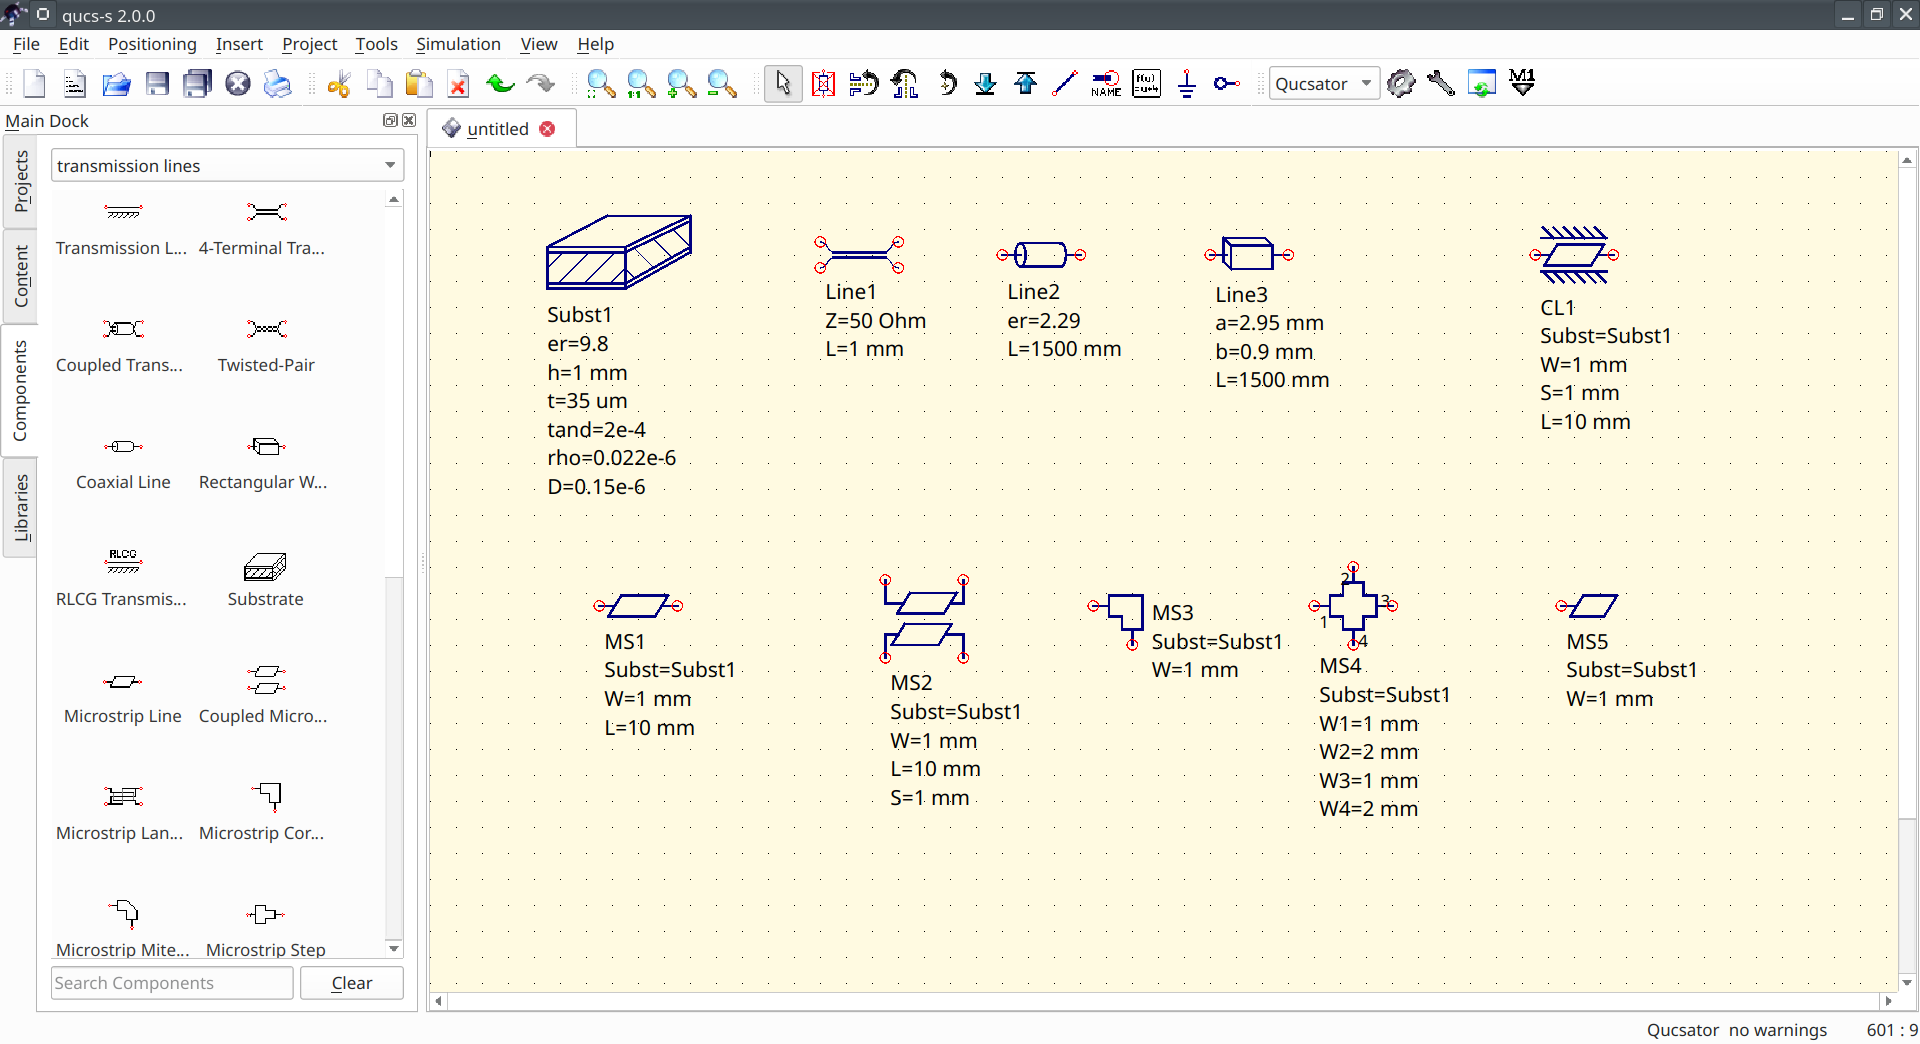
\includegraphics[width=\textwidth]{tlines.png}
    \end{center}
    \caption{Transmission lines models available for Qucsator backend} \label{fig:tlines}
    \end{figure}

Let's consider the basics of microstrip circuits simulation. Every microstrip line component requires to attach the substrate. The substrate is represented by special component too (Fig. \ref{fig:subst}). It is possible to define the substrate material properties and microstrip lines thickness. Substrate reference should be specified as the first parameter of all microstrip devices.

    \begin{figure}[!ht]
    \begin{center}
        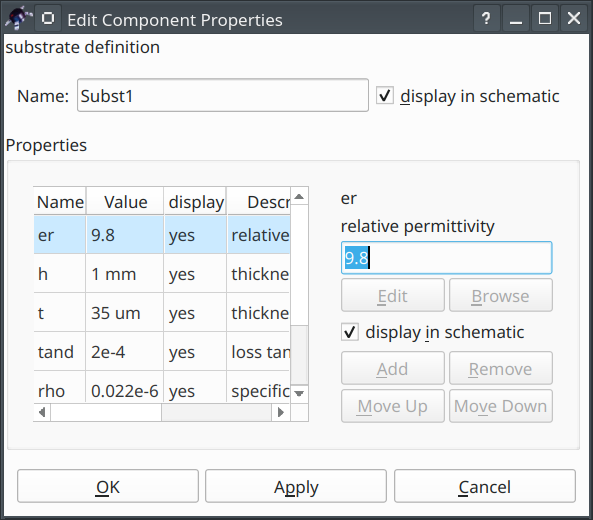
\includegraphics[width=0.4\textwidth]{substr.png}
    \end{center}
    \caption{Substrate properties definition} \label{fig:subst}
    \end{figure}

The simulation of the 1.5 GHz coupled microstrip bandpass filter is shown in the Fig. \ref{fig:mlin}. The schematic contains two ports P1 and P2 connected to input and output, two microstrip devices MS1 and MS2, and substrate Subst1. The S-parameter simulation definition has no difference to Ngspice and represented by a special component. The frequency range is defined from 1.3 to 1.7 GHz.

    \begin{figure}[!ht]
    \begin{center}
        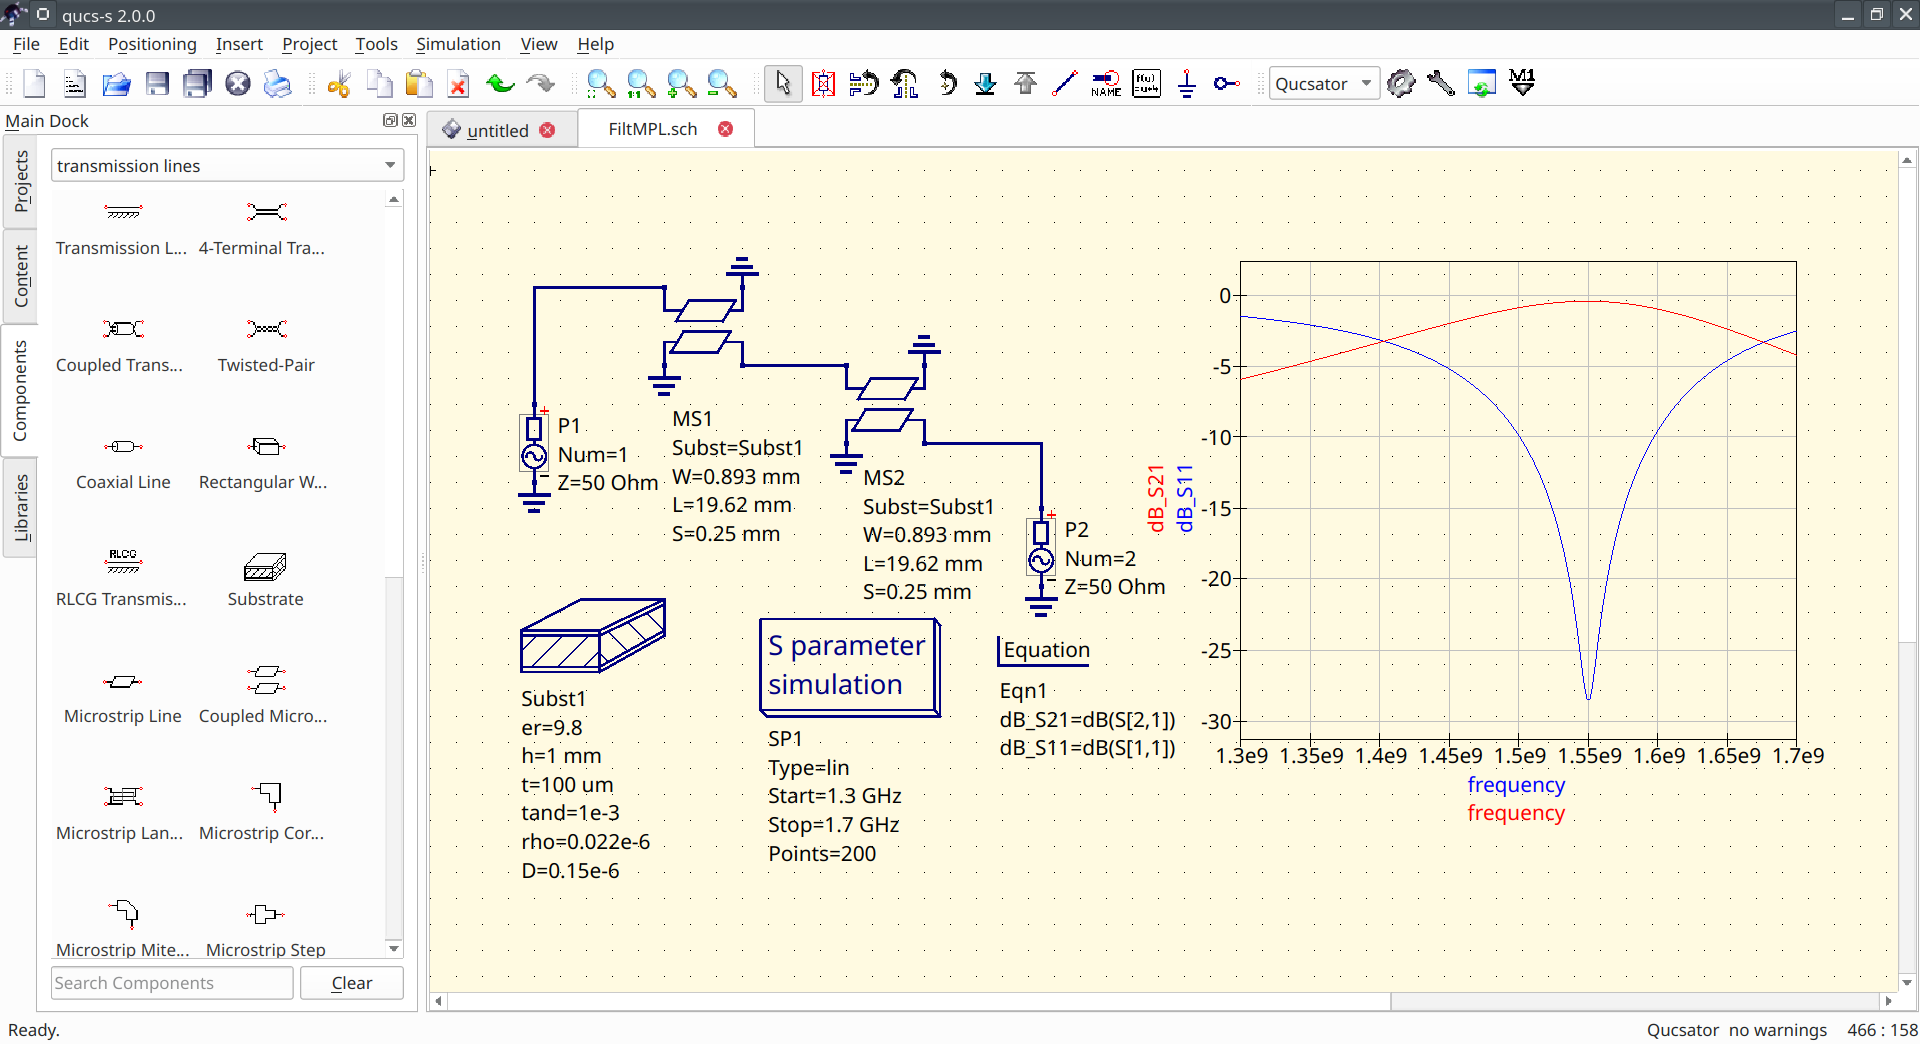
\includegraphics[width=0.8\textwidth]{filt_mlin.png}
    \end{center}
    \caption{Coupled microstrip bandpass filter simulation} \label{fig:mlin}
    \end{figure}

The schematic contains two equation that serves to express the S-parameters in Decibels using \verb|dB()| function. Keep in mind that equation syntax for Qucsator is different. Ngspice equations will not work with Qucsator. The S-parameter is represented in \verb|S[i,j]| form. For example \verb|S[2,1]| for $S_{21}$. Qucsator doesn't calculate Y and Z matrices automatically like Ngspice. You have to use the functions \verb|stoy()| and \verb|stoz()| for matrix conversion. Refer to Qucsator documentation for more details.

\section{Quick switching of the simulation kernel} \label{sec:quick_sw}

\subsection{Quick simulator selection}

Qucs-S supports a quick switching of the simulation kernel since the version 2.0.0. Application restart is not required anymore to apply this setting. The simulator could be selected at any time using the drop-down list on the toolbar Figure \ref{fig:sim_switch}. The simulator location must be configure using the application settings dialog Figure \ref{fig:sim_setup} and the specified simulator executable binary must exist. Otherwise the simulator will be not shown in the drop-down list on the toolbar and not available for selection. The list of the supported simulation kernels could be found in the section \ref{sec:intro}.

Also keep in mind that Qucs-S distribution doesn't provide any simulation kernels and simulators must be installed separately. If you are using Linux DEB package, the Ngspice will be installed automatically as the package dependency. This selection affects only analog simulation. The digital simulation kernel will be executed automatically if the schematic contains the digital simulation (see the section \ref{sec:digi}).

    \begin{figure}[!ht]
    \begin{center}
        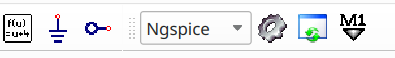
\includegraphics[width=0.66\textwidth]{sim_switch.png}
    \end{center}
    \caption{Simulator choose drop-down list} \label{fig:sim_switch}
    \end{figure}

\subsection{Incompatible components}

Some of devices may be incompatible with the selected simulation kernel. For example, microstrip lines are designed for Qucsator and are not available with Ngspice. Such devices will be not available for insertion in the schematic and will be grayed out (see Figure \ref{fig:grey}) on the schematic view. An appropriate warning will be shown if the user tries to simulate the schematic containing incompatible devices.

    \begin{figure}[!ht]
    \begin{center}
        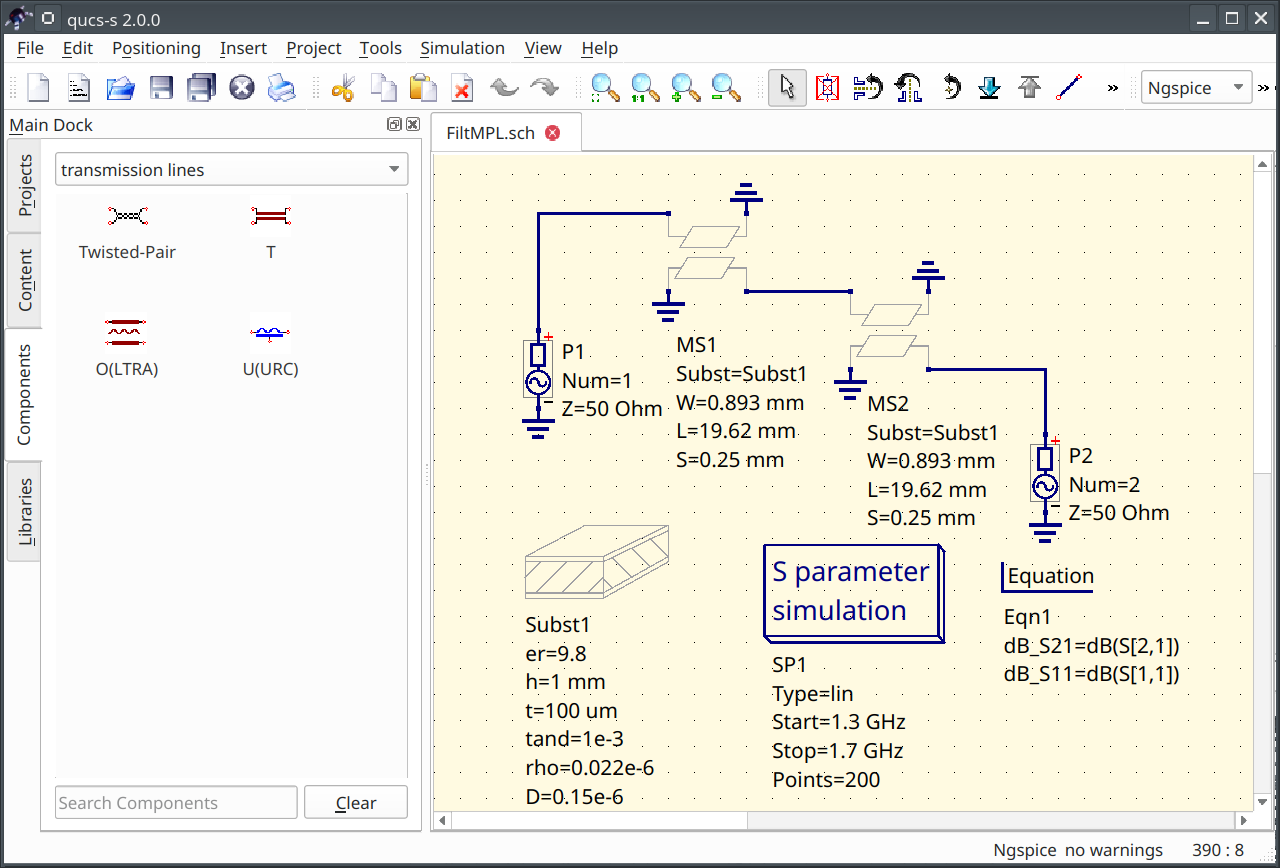
\includegraphics[width=0.8\textwidth]{ms_grey.png}
    \end{center}
    \caption{Schematic containing incompatible devices} \label{fig:grey}
    \end{figure}

\section{List of mathematical functions supported by Nutmeg equation}

The full list of the mathematical functions supported by Nutmeg equations could be found at the section 17.2 of the Ngspice manual. The next table shows the most frequently used functions. The input of all functions listed in the next table is a single vector representing voltage or current. Refer to the section 17 of the Ngspice manual for detailed description and information on additional functions.

\begin{table}[!ht]
\caption{The list of the most frequently used Nutmeg functions}
 \begin{tabularx}{\textwidth}{|r|X|}
\hline
Function & Description \\
\hline
mag & Magnitude of vector (same as abs(vector)) \\
ph & Phase of vector. \\
cph & Phase of vector. Continuous values, no discontinuity at $\pm\pi$ \\
unwrap & Phase of vector. Continuous values, no discontinuity at $\pm\pi$ Real phase vector in degrees as input \\
real & The real component of vector \\
imag & The imaginary part of vector\\
conj & The complex conjugate of a vector \\
db & Decibels $20 \log_{10}()$ of the vector \\
abs & The absolute value of vector (same as mag) \\
integ & Integrates over the given vector (versus the real component of the scale vector) \\
deriv & Calculates the derivative of the given vector \\
vecd & Compute the differential of a vector \\
group\_delay & Calculates the group delay $-d\phi/d\omega$ \\
\hline
\end{tabularx}
\end{table}

\section{Conclusion}

In this tutorial it was considered how to perform a first start setup of the Qucs-S with the Ngspice backend and make an AC and Transient simulation of the simple RC circuit. It was shown how to add postprocessor equations and waveforms plot. Refer to official Qucs-S and Ngspice documentation to learn more advanced simulation techniques.

\endinput




